\documentclass[a4paper, 12pt, twoside, openright]{book}
\addtolength{\oddsidemargin}{+1.3cm}
\addtolength{\evensidemargin}{-1.3cm}
%REMOVE ON PRINTING
%\linespread{1.3}
\usepackage[english, italian]{babel}
\usepackage{lipsum}
\usepackage[T1]{fontenc}
\usepackage[utf8]{inputenc}
\usepackage{fancyhdr}
\usepackage{float}
\usepackage{graphicx}
\usepackage{wrapfig}
\usepackage{siunitx} %per scrivere il simbolo °
\usepackage{verbatim} %per i commenti1
\usepackage{subcaption}
\usepackage{amsmath}
\usepackage[linesnumbered, ruled, vlined]{algorithm2e}
\setcounter{secnumdepth}{3}
\setcounter{tocdepth}{6}
\usepackage{multirow}
\usepackage{enumitem}
\usepackage{longtable}
\newcommand{\minitab}[2][l]{\begin{tabular}#1 #2\end{tabular}}
\usepackage{rotating}
\usepackage{url}
\DeclareMathOperator*{\argmax}{arg\,max}
\DeclareMathOperator*{\argmin}{arg\,min}

%\usepackage{booktabs,array}
%\usepackage{tikz}

%\usepackage{tabularx}

%\usepackage{chngcntr}
%\counterwithin{table}{section}

%------------------------------ colors
\usepackage[usenames,dvipsnames,table]{xcolor} % use colors on table and more
\definecolor{333}{RGB}{51, 51, 51} % define custom color
\definecolor{background}{RGB}{255, 254, 213}
\definecolor{comment}{RGB}{17,167,5}
\definecolor{keyword}{RGB}{195,47,8}
\definecolor{string}{RGB}{142,195,0}
\definecolor{number}{RGB}{90,84,84}
\definecolor{identifier}{RGB}{0,90,201}
\definecolor{commentAlg}{RGB}{36, 107, 206}
\definecolor{darkCell}{RGB}{36, 36, 36}
\definecolor{middleCell}{RGB}{128, 128, 128}

%------------------------------ source code
\usepackage{listings}

\lstset{
  basicstyle=\footnotesize\sffamily,
  commentstyle=\itshape\color{gray},
  captionpos=b,
  frame=shadowbox,
  language=HTML,
  rulesepcolor=\color{333},
  tabsize=2
}

\lstdefinestyle{code}{
  backgroundcolor=\color{background},
  basicstyle=\footnotesize\sffamily,
  commentstyle=\color{comment},
  frame=L,
  identifierstyle=\color{identifier},
  keywordstyle=\color{keyword},
  numbers=left,
  numbersep=10pt,
  numberstyle=\tiny\color{number},
  stringstyle=\color{string},
  showstringspaces=false,  
  stepnumber=1,
  tabsize=2
}

%------------------------------ define Abstract environment, missing in the 'book' class
\newenvironment{abstract}{
  \vspace*{\fill}
  \begin{center}%
    \bfseries\abstractname
  \end{center}}%
  {\vfill} % change Abstract title

%------------------------------ active url
\usepackage{url}
\renewcommand{\UrlFont}{\color{black}\small\ttfamily} % active ref
%------------------------------ macros
\newcommand{\sectionname}{Section} % define Section ref
\newcommand{\subsectionname}{Sub-section} % define Sub-section ref
\renewcommand*\arraystretch{1.4} % tables padding

%acronimi
\usepackage[printonlyused]{acronym}

%Rules in tables
\usepackage{booktabs}

%Formatted quote
\newcommand{\myquote}[2]{
\begin{quote}
	\textbf{\Large ``}{\textit{#1}}\textbf{\Large ''}\\
	\textbf{#2}\\\\
\end{quote}
}

%Formatted item with description
\newcommand{\descItem}[2]{\item{\textbf{#1}\\#2}}

%Formatted item with description
\newcommand{\myBibItem}[4]{\bibitem{#1}#2, "#3" in \emph{#4}.}

\newcommand{\myBibRef}[5]{\bibitem{#1}#2, \href{#3}{"#4"}, \emph{#5}.}

%Cell with vertical text
\newcommand{\verticalCell}[2]{\multirow{#1}{*}{\rotatebox[origin=c]{90}{#2}}}

%Tab Item Cell
\newcommand{\itemCell}[1]{\textbullet\ {#1}}

\newcommand{\itemCellTab}[1]{\hspace{0.5cm}\textbullet\ {#1}}

\newcommand{\key}[1]{\textbf{\color{blue}{#1}}}

\newcommand{\myref}[2]{\textbf{#1 \ref{#2}}}

\usepackage[colorlinks=true, linkcolor=black, citecolor=blue, urlcolor=black]{hyperref}

\begin{document}
\frontmatter
%\addtolength{\oddsidemargin}{-0.7cm}
\begin{titlepage} %------------------------------ TITLE PAGE
\begin{center}
\begin{minipage}{\textwidth}
\begin{center}
  \begin{table}[H]
  \centering  
  \begin{tabular}{p{\textwidth}}
  \multicolumn{1}{c}{\scshape{\bfseries{\large{Università Degli Studi Di Padova}}}}\\
  \hline
  \multicolumn{1}{c}{\scshape{\bfseries{\large{Department~of~Information~Engineering}}}}\\
  \end{tabular}
  \end{table}
\end{center}
\end{minipage}\\
\Large{\textit{Master~Degree~in~Computer~Engineering}} \\
\vspace{0.5cm}
\begin{minipage}{.25\textwidth}
  
\includegraphics[width=\textwidth]{./Images/unipd-bn}
\end{minipage}

\vspace{1.0cm}
\scshape{\Large{\bfseries{AcCAPPCHA:\\}}}
\scshape{\large{\bfseries{Design, Development and Security Analysis\\}}}
\scshape{\large{\bfseries{of an Invisible CAPPCHA based on\\}}}
\scshape{\large{\bfseries{an acoustic side-channel\\}}}
\vspace{0.2cm} \linespread{1} 
\scshape{\large{\bfseries{}}}
\end{center}

\vspace{3cm}
\begin{normalsize}
\begin{flushleft}
  %\hspace{45pt} \textit{Laureando} \hspace{160pt} \textit{Relatore}\\
  
  \hspace{62pt} \textbf{\textit{Candidate}} \hspace{130pt} \textbf{\textit{Supervisor}}\\
  \vspace{5pt}
  \hspace{27pt} {Di Nardo Di Maio Raffaele} \hspace{65pt} {Prof. Migliardi Mauro}\\
\end{flushleft}
\end{normalsize}

\vfill
\begin{center}
\textsc{DD-MM-2021}
\hspace{-0.2cm}
\line(1, 0){360}

\textsc{Accademic Year 2020-2021}
\end{center}
\end{titlepage}
\cleardoublepage % make left page blank
\thispagestyle{empty}
%\pagevalues
\addtolength{\oddsidemargin}{+0.7cm}
\begin{titlepage} %------------------------------ TITLE PAGE
\begin{center}
\vbox to0pt{\vbox to\textheight{\vfill 
\includegraphics[width=11.5cm]{./Images/unipd-light} \vfill}\vss}

\begin{minipage}{.20\textwidth}
  
\includegraphics[height=2.5cm]{./Images/unipd-bn}
\end{minipage}\begin{minipage}{.90\textwidth}
  \begin{table}[H]
  \begin{tabular}{l}
  \scshape{\Large{\bfseries{University of Padova}}} \\
  \hline
  \scshape{\Large{Engineering~Departement}} \\
  \end{tabular}
  \end{table}
\end{minipage}

\vspace{1cm}
\emph{\Large{Computer~Engineering~Master~Degree}} \\
\vspace{1.5cm}
\scshape{\Large{\bfseries{AcCAPPCHA:\\}}}
\scshape{\large{\bfseries{Design, Development and Security Analysis\\}}}
\scshape{\large{\bfseries{of an Invisible CAPPCHA based on\\}}}
\scshape{\large{\bfseries{an acoustic side-channel\\}}}
\vspace{0.2cm} \linespread{1} 
\scshape{\large{\bfseries{}}}
\end{center}

\vfill
\begin{normalsize}
\begin{flushleft}
  %\hspace{45pt} \textit{Laureando} \hspace{160pt} \textit{Relatore}\\
  \hspace{65pt} \textit{Candidate} \hspace{130pt} \textit{Supervisor}\\
  \vspace{5pt}
  \hspace{25pt} \large{\textbf{\footnotesize{Di Nardo Di Maio Raffaele}}} \hspace{55pt} \large{\textbf{\footnotesize{Prof. Migliardi Mauro}}}\\
\end{flushleft}
\end{normalsize}

\vfill
\begin{center}
\textsc{DD-MM-2021}
\hspace{-0.2cm}
\line(1, 0){360}

\textsc{Accademic Year 2021-2022}
\end{center}
\end{titlepage}
\cleardoublepage % make left page blank
\thispagestyle{empty}
\null
\vspace{2cm}
\begin{flushright}
     To my parents, who always help\\
   me to be happy doing what I love\\
and support me in reaching my goals.
\end{flushright}
\vfill
\cleardoublepage % make left page blank
\null
\vspace{2cm}
\thispagestyle{empty}
\myquote{Most people assume that once security software is installed, they're protected. This isn't the case. It's critical that companies be proactive in thinking about security on a long-term basis.}{Kevin Mitnick}
\myquote{You have to learn the rules of the game. And then you have to play better than anyone else.}{Albert Einstein}
\myquote{Si come il ferro s'arrugginisce sanza esercizio, e l'acqua si putrefà o nel freddo s'addiaccia, così lo 'ngegno sanza esercizio si guasta.}{Leonardo da Vinci}
\vfill
\null
%\begin{abstract} %------------------------------ ABSTRACT
%\addcontentsline{toc}{chapter}{Abstract}
%\markboth{}{} % remove header
%\thispagestyle{empty}
%This is the abstract
%\end{abstract}

%%\begin{abstract} %------------------------------ ABSTRACT
%\addcontentsline{toc}{chapter}{Abstract}
%\markboth{}{} % remove header
%\thispagestyle{empty}
%This is the abstract
%\end{abstract}

%%\begin{abstract} %------------------------------ ABSTRACT
%\addcontentsline{toc}{chapter}{Abstract}
%\markboth{}{} % remove header
%\thispagestyle{empty}
%This is the abstract
%\end{abstract}

%\input{Chapters/Abstract.tex}

\begingroup
  %------------------------------ CONTENTS
  \makeatletter
  \let\ps@plain\ps@empty
  \makeatother
  \tableofcontents  
  \clearpage
\endgroup

\mainmatter
\chapter{Introduction}
\begin{itemize}
\item{\textbf{Arithmetic}\\
}
\item{\textbf{Audio-based}\\
}
\item{\textbf{Game-based}\\
}
\item{\textbf{Image-based}\\
}
\item{\textbf{Puzzle-based}\\
}
\item{\textbf{Text-based}\\
}
\item{\textbf{Video-based}\\
}
\end{itemize}

\begin{table}
\centering \footnotesize
\renewcommand*\arraystretch{1.3}
\begin{tabular}{cll}
\hline
{\textbf{CAPTCHA type}} & {\textbf{Usability issues}} & {\textbf{Security}}\\
\hline
\textit{Arithmetic} & {} & {}\\
\hline
\textit{Audio-based} & {
  \begin{minipage} [t] {0.4\textwidth}
  Issues of recognition:
      \begin{itemize}
        \item{Previous knowledge of English dictionary by the user.}
        \item{Some character sounds very similar to others.}
       \end{itemize} 
  \end{minipage}
} & {}\\
\tabularnewline
\hline
\textit{Game-based} & {} & {}\\
\hline
\textit{Image-based} & {
 \begin{minipage} [t] {0.4\textwidth}
Difficulty of identification of images caused by:
      \begin{itemize}
        \item{Blur of images.}
        \item{Low vision condition.}
       \end{itemize} 
  \end{minipage}
} & {}\\
\tabularnewline
\hline
\multirow{2}{*}{\textit{Puzzle-based}} & {It takes too much time to solve the puzzle} & {}\\
{} & {and to identify the arrangement of puzzles.} & {}\\
\hline
\textit{Text-based} & {
  \begin{minipage} [t] {0.4\textwidth}
	Many problems have to be solved by user:
      \begin{itemize}
        \item{Multiple fonts.}
        \item{Font size.}
        \item{Blurred Letters}
        \item{Wave Motion.}
       \end{itemize} 
  \end{minipage}
}
& {It can be identified by OCR (Optical Character Recognition) technique.}\\
\tabularnewline
\hline
\textit{Video-based} & {
Issues downloading videos to find correct} & {}\\
{} & {captcha because of large size of files.} & {}\\

\end{tabular}
\end{table}
\chapter{State of the Art}\label{chapter:StateOfArt}
CAPTCHA is the acronym of \textit{"Completely Automated Public Turing-test-to-tell Computers and Humans Apart"} and it's a challenge born from these two components\cite{types_CAPTCHA}:
\begin{enumerate}
\descItem{Human-Computer Interaction (HCI)}
{it is a research field that studies the computer technology, looking at the interfaces between the users and the machines. A human can interact with a machine at several levels:
\begin{itemize}
	\item{Task level}
	\item{Semantic level}
	\item{Syntactic level}
	\item{Interactive level}
	\item{Physical devices level}
\end{itemize}
This discipline tries to analyse the ways in which a human can process data, matching the user's needs and interests. According to cognitive psychology studies, the human interaction with the machine is based on:
\begin{itemize}
	\item{Reasoning}
	\item{Problem solving}
	\item{Skill acquisition}
	\item{Error}
\end{itemize}   
}
\descItem{Human Interactive Proof (HIP)}
{it's a proof used to classify machines and humans looking at a specific type of interaction, that is simple to be done by a human instead of a bot. The main goals of the test are:
\begin{itemize}
	\item{To differentiate the humans from the computers}
	\item{To differentiate a category of the humans}
	\item{To differentiate a specific human from the category of humans}
\end{itemize}
HIP consists of a test program administered to humans and computers. The main problem of this proof is that the complexity of the task is often very complex and only a specific group of humans can usually solve the test.\\
Historically the most widely known version is the cognitive one defined by Alan Turing. The Turing test is used to determine how much a machine is capable of thinking like a human. The experiment involves three figures: a human examiner, a human and a machine. The examiner asks some questions to the other figures and, after a fixed amount of time, he evaluates if the two answers were different or not.\\
If they were similar, with respect to the point of view of the examiner, the machine is classified as an AI (Artificial Intelligence). The test is very reliable if each question could have many possible answers.}
\end{enumerate}
The design of CAPTCHA challenges takes inspiration from the previous components because its goal is to establish if the user is a bot or a human. A bot is usually an advanced program that exploits some AI techniques and pretends to be a human. In the endeavor of foiling bots that are getting every day smarter and more sophisticated, a CAPTCHA challenge sometimes is so complex that a human user can't solve it. For this reason and in order to guarantee an high level of security, a CAPTCHA has to satisfy the following requirements:
\begin{itemize}
	\item{There exists only one solution of a CAPTCHA and it shouldn't depend on the user's language and/or age;}
	\item{The solution of a CAPTCHA must be easy for the humans and hard for the bots. In fact humans should solve it in no longer than 30 seconds with very high success rate (30 seconds are usually considered too much time to solve a CAPTCHA);}
	\item{The creation of a CAPTCHA shouldn't affect the user privacy.}
\end{itemize}
Over the year, the CAPTCHAs must satisfy more and more requirements and the challenges become more and more complex reducing the usability of them. For this reason, a new generation of CAPTCHAs, that we define modern CAPTCHAs, has been developed in the last years. The new challenges are related to a good exploitation of the biometrics and the sensors of modern devices. In addition, machine learning techniques and side-channel information are used to evaluate the user behaviour instead of generating challenges based on cognitive capabilities. 

%\vspace{4cm}
\section{Traditional CAPTCHAs}
The traditional CAPTCHAs are based on the knowledge and the correct insertion of the solution by the user. These CAPTCHA schemes are designed to leverage character recognition, image analysis and speech recognition to guarantee that the challenges will successfully block bots.\\
The main types of traditional CAPTCHAs, namely Audio-based CAPTCHAs, Game-based CAPTCHAs, Image-based CAPTCHAs, Math CAPTCHAs, Slider CAPTCHAs, Text-based CAPTCHAs and Video-based CAPTCHAs, are described in the following sections but the details about specific implementations can be found in the article of Walid Khalifa Abdullah Hasan\cite{survey_advanced_CAPTCHA}. With respect to user experience, the most enjoyable traditional CAPTCHAs are usually the game-based and image-based ones while the most frustrating CAPTCHA is the text-based one\cite{usability_CAPTCHA}. A summary of usability and security issues, explained in the following sections, is also reported in \myref{Table}{soa:traditional_table}.

\subsection{Audio-based CAPTCHAs}
This type of CAPTCHAs asks the user to type the words contained in an audio file (see \myref{Figure}{soa:audio_CAPTCHA}). It's developed for vision-impaired users. Audio-based CAPTCHAs usually have problems in usability related to the language dictionary, from which the words are taken, and the similarity of sound for several words. This CAPTCHA is a hard task even for blind users, in fact  during an experiment only 46\% of the challenges were solved by the participants\cite{usability_audio}.\\
One of the most popular Audio-Based CAPTCHAs is \textit{Audio reCAPTCHA}, developed at Carnegie Mellon University and then bought by Google. In this scheme, the user needs to recognize and write a set of 8 spoken characters from a noisy audio file with several background voices. If the user makes a mistake, the test declares that he's a bot.\\
Audio-based CAPTCHAs are vulnerable to many Automatic Speech Recognition (ASR) programs\cite{improving_audio} but also Deep Learning techniques (e.g. DeepCRACk\cite{DeepCRACk}). A good overview about results, obtained by several classification methods, is described in the work of Jennifer Tam et al.\cite{break_audio}.
\begin{figure}[h]
     \centering
     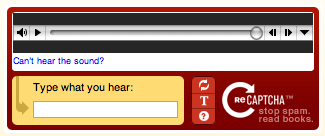
\includegraphics[width=.4\linewidth]{Images/StateOfArt/audio_CAPTCHA}
     \caption{\footnotesize{Example of audio-based CAPTCHA.}}\label{soa:audio_CAPTCHA}
\end{figure}

\subsection{Game-based CAPTCHAs}
This type of CAPTCHAs performs the verification of the user identity through a set of several kinds of games (see \myref{Figure}{soa:game}). The strength of Game-based CAPTCHAs is related to the the rules of the game that only humans can understand.\\
There exists an implementation of these CAPTCHAs, called \textit{Dynamic Cognitive Game (DCG)}, that is usually developed using Flash, HTML5 and JavaScript. These technologies download the game code to the client and execute it locally.\\
The code of these challenges must be the obfuscated to prevent that the source file could be analysed by an attacker. In fact, the obfuscation guarantees that the source code can not be stored on different internet domains. However for example, there exists a bot attack, called \textit{Stream Relay Attack}, that obtains good results bypassing these challenges \cite{game_CAPTCHA} (see \myref{Section}{soa:security_CAPTCHAs}).
\begin{figure}[h]
     \centering
     \begin{subfigure}[b]{0.48\textwidth}
         \centering
         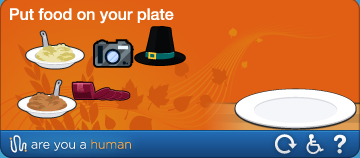
\includegraphics[width=.9\linewidth]{Images/StateOfArt/game_CAPTCHA}
     \end{subfigure}
     \hfill
     \begin{subfigure}[b]{0.48\textwidth}
         \centering
         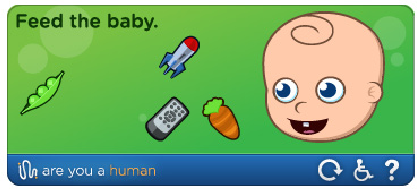
\includegraphics[width=.9\linewidth]{Images/StateOfArt/game_CAPTCHA2}
     \end{subfigure}
		
	 \begin{subfigure}[b]{0.55\textwidth}
         \centering
         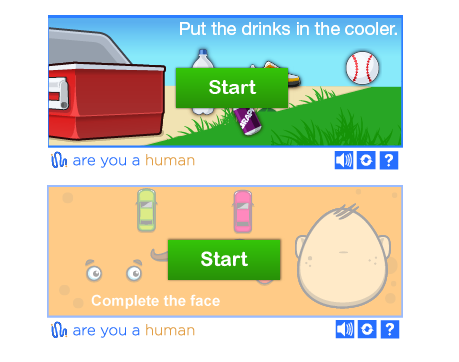
\includegraphics[width=\linewidth]{Images/StateOfArt/game_CAPTCHA3}
     \end{subfigure}
     \caption{\footnotesize{Examples of game-based CAPTCHAs.}}
     \label{soa:game}
\end{figure}

\subsection{Image-based CAPTCHAs}
Image-based CAPTCHAs is based on a written text that describes a task related to the evaluation of some images. The user must understand the action and he passes the test if he performs it in the right way. This type of CAPTCHAs can be categorized into the following classes, looking at the task that the user needs to perform:
\begin{itemize}
\descItem{Click-based CAPTCHAs}
{this type of CAPTCHAs shows an image and a text that explains where the user needs to click (see \myref{Figure}{soa:click_CAPTCHA}).
\begin{figure}[h]
     \centering
     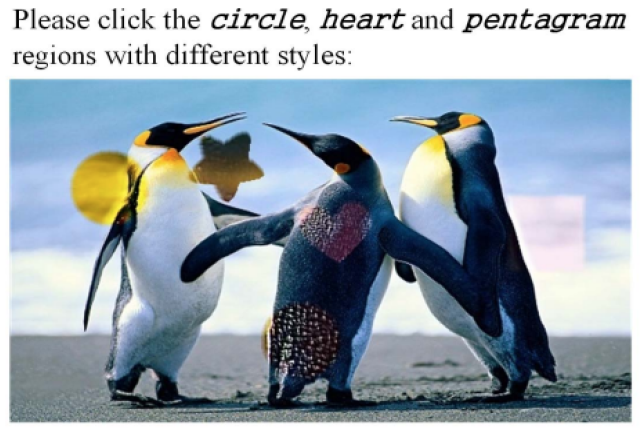
\includegraphics[width=.45\linewidth]{Images/StateOfArt/click_CAPTCHA}
     \caption{\footnotesize{Example of click-based CAPTCHA.}}\label{soa:click_CAPTCHA}
\end{figure}
}
\descItem{Sliding image-based CAPTCHAs}
{this type of CAPTCHAs asks the user to use the slider to solve an image-based challenge such as adjusting the orientation of an image, selecting the correct form of an image, or moving a fragment of an image to the correct location (see \myref{Figure}{soa:sliding_image}).
\begin{figure}[h]
     \centering
     \begin{subfigure}[b]{0.48\textwidth}
         \centering
         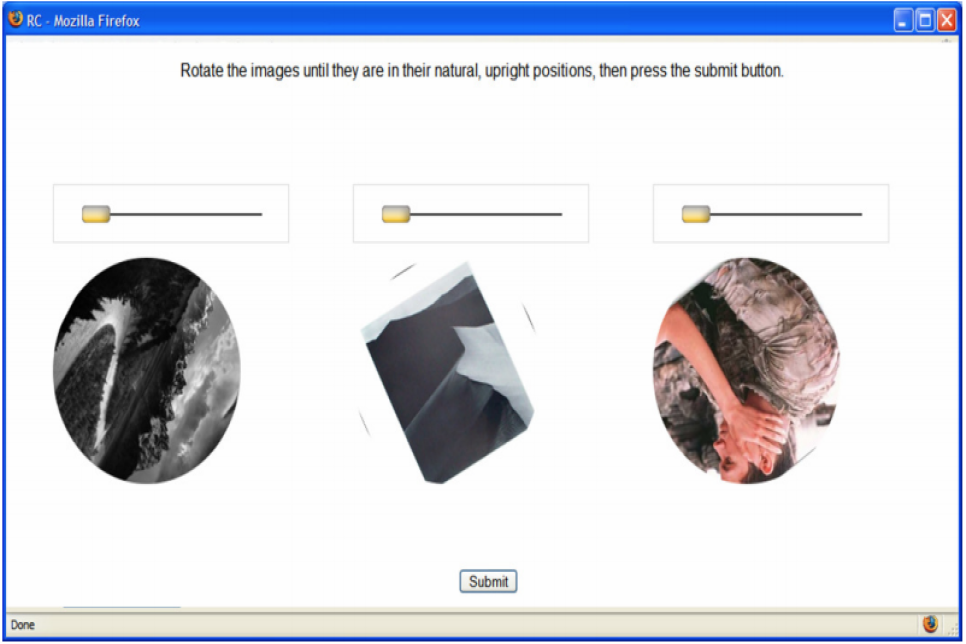
\includegraphics[width=.9\linewidth]{Images/StateOfArt/sliding_image_CAPTCHA}
	     \caption{\footnotesize{Orientation based.}}
     \end{subfigure}
     \hfill
     \begin{subfigure}[b]{0.48\textwidth}
         \centering
         
\includegraphics[width=.9\linewidth]{Images/StateOfArt/sliding_image_CAPTCHA2}
	     \caption{\footnotesize{Form based.}}
     \end{subfigure}
     \caption{\footnotesize{Examples of sliding image-based CAPTCHAs.}}
     \label{soa:sliding_image}
\end{figure}
}
\descItem{Drag \& Drop-based CAPTCHAs}
{this type of CAPTCHAs usually asks the user to complete a visual puzzle, created by dividing a given image in a set of pieces\cite{survey_CAPTCHA} (see \myref{Figure}{soa:puzzle}).\\
The task isn't easy for users because this type of CAPTCHAs takes more time to solve the puzzle but the security level is very high\cite{survey_CAPTCHA}. To improve the usability of the CAPTCHA, there exists a version of the puzzle-based CAPTCHA in which the user needs to insert only some pieces of the puzzle instead to complete it (see \myref{Figure}{soa:puzzle2}).
\begin{figure}[h]
     \centering
     \begin{subfigure}[b]{0.48\textwidth}
         \centering
         
\includegraphics[width=.6\linewidth]{Images/StateOfArt/puzzle_CAPTCHA}
         \caption{\footnotesize{Completing the puzzle.}}
         \label{soa:puzzle}
     \end{subfigure}
     \hfill
     \begin{subfigure}[b]{0.48\textwidth}
         \centering
         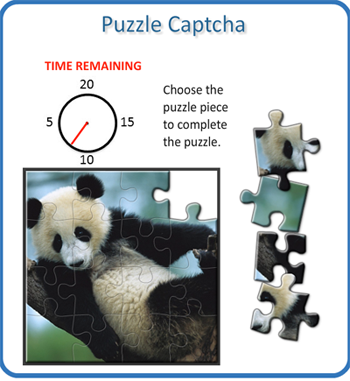
\includegraphics[width=.6\linewidth]{Images/StateOfArt/puzzle_CAPTCHA2}
         \caption{\footnotesize{Inserting only some pieces.}}
        \label{soa:puzzle2}
     \end{subfigure}
     \caption{\footnotesize{Examples of puzzle-based CAPTCHAs.}}
\end{figure}
}
\descItem{Selection-based CAPTCHAs}
{the user usually needs to select the images that contain a requested subject. The set of images, on which the user needs to identify the subject, can be created in several ways, for example:
\begin{itemize}
\item{An image is divided into a set of sub-squares and each of them is a candidate image (see \myref{Figure}{soa:selection})}
\item{There are many images, each one with a unique different subject (see \myref{Figure}{soa:selection2})}
\end{itemize}
This type of CAPTCHAs is vulnerable to different Object Recognition techniques developed for Computer Vision purposes.\\
An extension of this type of CAPTCHAs, called \textit{FaceDCAPTCHA}, has been introduced\cite{FaceDCAPTCHA} and it incorporates elements of face detection. The human brain is very effective in the process of natural face segmentation even if there are complex backgrounds. In fact, this approach increases the security efficiency because the Computer Vision programs can easily detect if there is a face, e.g. Viola-Jones algorithm\cite{Viola_Jones}, but they have many problems understanding if the photographs of the faces are real or not.\\
One of the most difficult challenges, to be performed by a computer, is the detection of faces, fingerprints and eyes in an image. For this reason the previous idea has been used to to develop a new version of image-based CAPTCHA, called \textit{MB CAPTCHA}\cite{MB_CAPTCHA}.
\begin{figure}[h]
     \centering
     \begin{subfigure}[b]{0.48\textwidth}
         \centering
         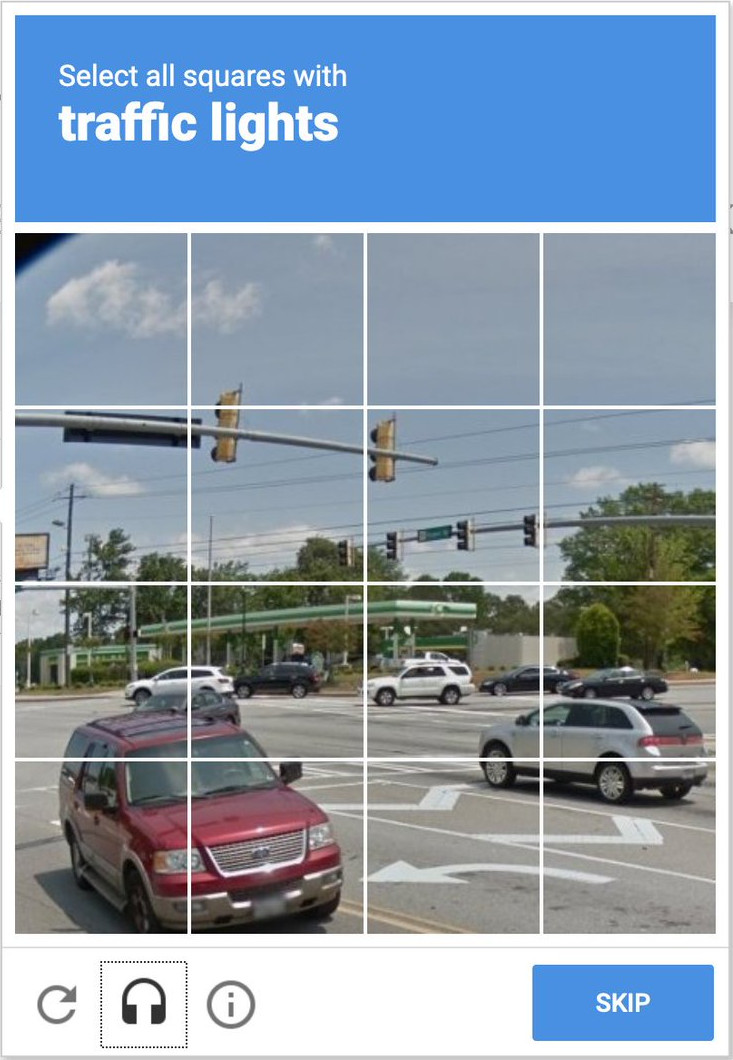
\includegraphics[width=.68\linewidth]{Images/StateOfArt/selection_CAPTCHA}
         \caption{\footnotesize{With an image divided in sub-squares.}}
         \label{soa:selection}
     \end{subfigure}
     \hfill
     \begin{subfigure}[b]{0.48\textwidth}
         \centering
         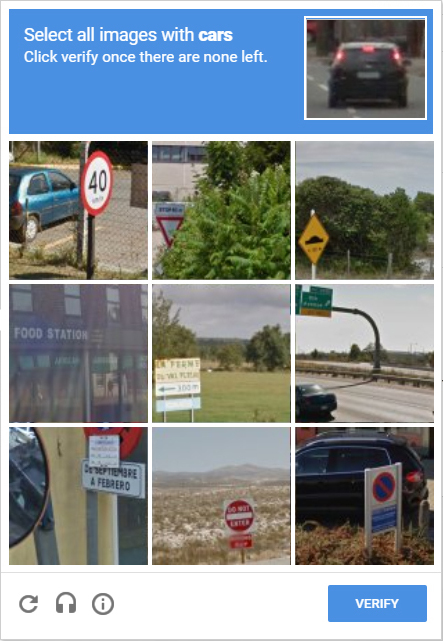
\includegraphics[width=.68\linewidth]{Images/StateOfArt/selection_CAPTCHA2}
         \caption{\footnotesize{With several images.}}
        \label{soa:selection2}
     \end{subfigure}
     \caption{\footnotesize{Examples of selection-based CAPTCHAs.}}
\end{figure}
}
\descItem{Interactive-based CAPTCHAs}
{the user needs to discover a secret position in an image using mouse movements or swiping gestures
\begin{figure}[h]
     \centering
     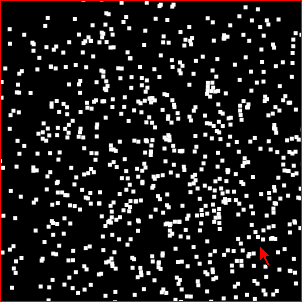
\includegraphics[width=.4\linewidth]{Images/StateOfArt/interactive_CAPTCHA}
     \caption{\footnotesize{Example of interactive-based CAPTCHA.}}\label{soa:interactive_CAPTCHA}
\end{figure}
}
\end{itemize}

\subsection{Math CAPTCHAs}
Looking to a math operation, specified in a frame, the user needs to insert the result in a text field. The operation is written in plain text or, to improve the security of this challenge, it's warped like text-based CAPTCHAs (see \myref{Figure}{soa:arithmetic}). These classical math-CAPTCHAs, also known as \textit{arithmetic CAPTCHAs}, are vulnerable to OCR (Optical Character Recognition) techniques.\\
\begin{figure}[h]
     \centering
     \begin{subfigure}[b]{0.48\textwidth}
         \centering
         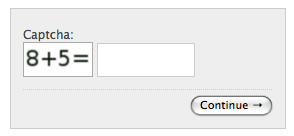
\includegraphics[width=.7\linewidth]{Images/StateOfArt/math_CAPTCHA}
         \caption{\footnotesize{With plain text.}}
     \end{subfigure}
     \hfill
     \begin{subfigure}[b]{0.48\textwidth}
         \centering
         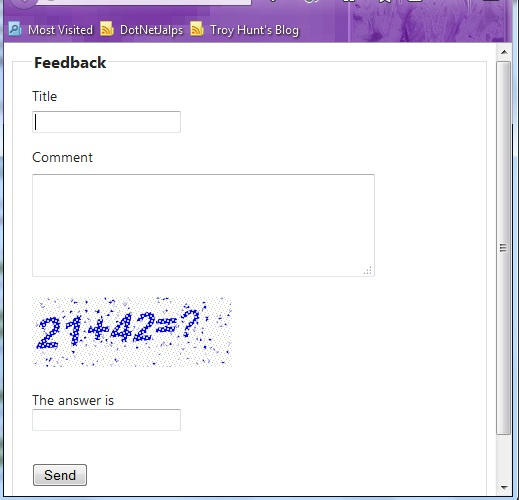
\includegraphics[width=.7\textwidth]{Images/StateOfArt/math_CAPTCHA2}
         \caption{\footnotesize{With wrapped text.}}
     \end{subfigure}
		\caption{\footnotesize{Example of arithmetic CAPTCHAs.}}
		\label{soa:arithmetic}
\end{figure}
An advanced version of this CAPTCHA is used in the Quantum Random Bit Generator Service (QRBGS) sign-up Web Page\cite{math_CAPTCHA} (see \myref{Figure}{soa:QRBGS}). This type of CAPTCHA asks the user to solve an advanced math expression. It prevents the use of free or commercial OCR techniques because many mathematical symbols are not considered in the traditional detection algorithms. Hence many math symbols are wrongly translated by bot programs and the challenge is very secure. However, this CAPTCHA is vulnerable to side-channel attacks \cite{math_CAPTCHA} and it's very complex for normal users. In fact many people can't solve it correctly because the required level of math knowledge is very high and not very common.
\begin{figure}[h]
     \centering
     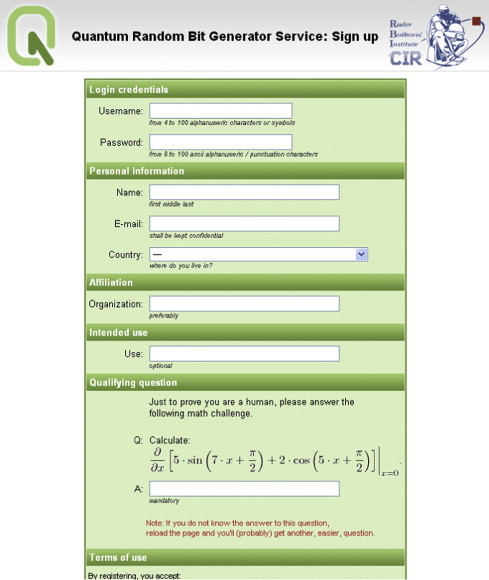
\includegraphics[width=.4\linewidth]{Images/StateOfArt/QRBGS}
     \caption{\footnotesize{Example of Quantum Random Bit Generator Service (QRBGS) sign-up Web Page \cite{math_CAPTCHA}.}}\label{soa:QRBGS}
\end{figure}

\subsection{Slider CAPTCHAs}
Slider CAPTCHAs ask users to move a slider across the screen. The image recognition is not part of the challenge.\\
The most popular CAPTCHAs of this type are the following:
\begin{itemize}
\descItem{CAPTCHA used by Taobao.com}{it asks the user to drag the slider from the start to the end of the sliding bar to verify his identity (see \myref{Figure}{soa:slider}).}
\descItem{CAPTCHA used by TheyMakeApps.com}{it asks the user to move the slider to the end of the line to submit a form\cite{sliding_CAPTCHA} (see \myref{Figure}{soa:slider2}).}
\end{itemize}
Over the years several implementations of this type of CAPTCHAs have been bypassed with a simple JavaScript code and puppeteer.
\begin{figure}[h]
     \centering
     \begin{subfigure}[b]{0.48\textwidth}
         \centering
         
\includegraphics[width=.8\linewidth]{Images/StateOfArt/taobao_CAPTCHA}
                  \caption{\footnotesize{Example of TaoBao.com CAPTCHA.}}
         \label{soa:slider}
     \end{subfigure}
     \hfill
     \begin{subfigure}[b]{0.48\textwidth}
         \centering
         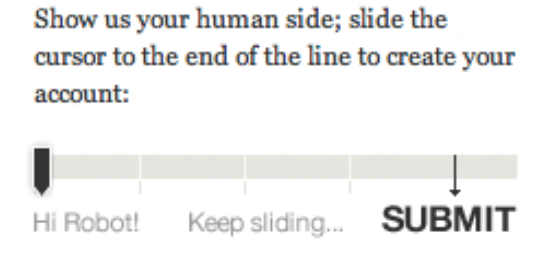
\includegraphics[width=.8\linewidth]{Images/StateOfArt/theyMakeApps_CAPTCHA}
         \caption{\footnotesize{Example of TheyMakeApps.com CAPTCHA.}}
        \label{soa:slider2}
     \end{subfigure}
     \caption{\footnotesize{Examples of slider CAPTCHAs.}}
\end{figure}

\subsection{Text-based CAPTCHAs}
In text-based CAPTCHA schemes a random series of warped characters and/or numbers is displayed on the screen inside an image (see \myref{Figure}{soa:text_CAPTCHA}). The user needs to understand which are the characters that composes the sequence and then he types them inside a text-field. The most known classes of text-based CAPTCHAs are:
\begin{itemize}
\descItem{2D}{the warped characters of the text are placed and oriented in a 2D plane, parallel to the screen plane. The image of the 2D plane is used in the challenge.}
\descItem{3D}{each warped character of the text is mapped into a 3D model of the character and then is placed and oriented in a 3D plane in the space. A 2D image of the 3D space is taken from a specific point of view and it's used in the challenge.}
\end{itemize}
This type of CAPTCHAs is vulnerable to several attacks, related to Computer Vision techniques:
\begin{itemize}
\item{OCR techniques\cite{OCR}}
\item{Segmentation techniques (e.g. DECAPTCHA\cite{DECAPTCHA})}
\item{Machine Learning and Deep Learning techniques}
\end{itemize}
In the design phase of a text-based CAPTCHA there are many issues, related to Computer Vision attacks, to be considered. For each of them, there is usually a solution in the design phase of the CAPTCHA that reduces the probability that the challenge will be broken by a bot\cite{DECAPTCHA}.
\begin{figure}[h]
     \centering
     
\includegraphics[width=.55\linewidth]{Images/StateOfArt/text_CAPTCHA}
     \caption{\footnotesize{Example of text-based CAPTCHA.}}\label{soa:text_CAPTCHA}
\end{figure}

\subsection{Video-based CAPTCHAs}
This type of CAPTCHAs isn't very common because it requires the download of a very large file\cite{survey_advanced_CAPTCHA}. The traditional video-based CAPTCHA is composed by a video in which a sliding text is shown (see \myref{Figure}{soa:video}). The user needs to type this message in a text field to pass the challenge. Some implementations of this type of CAPTCHAs are vulnerable to machine learning attacks.\\
Another version of the CAPTCHA is \textit{Motion CAPTCHA}\cite{Motion_CAPTCHA}, developed by M. Shirali-shahreza and S. Shirali-shahreza, in which the user needs to watch a video. Then he needs to select which action was performed in the played file, choosing it from multiple answers (see \myref{Figure}{soa:video2}). The strength of these implementations of CAPTCHAs is in the relationship between the multiple choices of the answer\cite{video_attack}.\\
A similar implementation of the previous version is the one developed by Kluever et al. in which the user watches a video and then he needs to write three words that describe what he sees\cite{video_desc}. The same authors created a tag frequency-based attack to evaluate the security of their CAPTCHA scheme and they achieve a success rate of 13\%.
\begin{figure}[h]
     \centering
     \begin{subfigure}[b]{0.48\textwidth}
         \centering
         
\includegraphics[width=\linewidth]{Images/StateOfArt/video_CAPTCHA}
         \caption{\footnotesize{Example of sliding text in video.}}
         \label{soa:video}
     \end{subfigure}
     \hfill
     \begin{subfigure}[b]{0.48\textwidth}
         \centering
         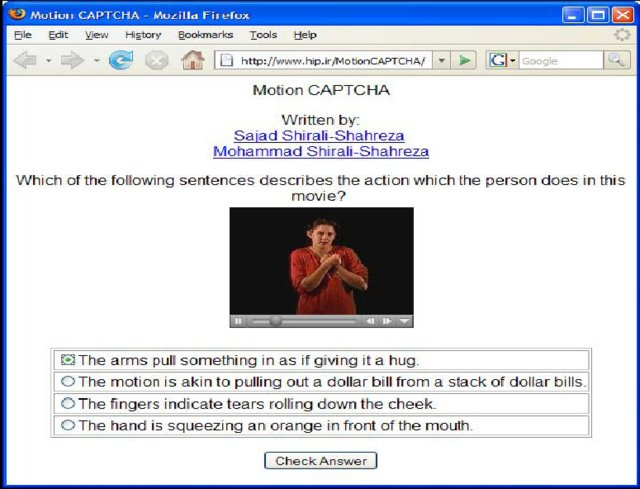
\includegraphics[width=\linewidth]{Images/StateOfArt/video_CAPTCHA2}
         \caption{\footnotesize{Example of Motion CAPTCHA\cite{Motion_CAPTCHA}.}}
        \label{soa:video2}
     \end{subfigure}
     \caption{\footnotesize{Examples of video-based CAPTCHAs.}}
\end{figure}

\section{Modern CAPTCHAs}
The type of CAPTCHAs and authentication mechanisms, described in the following sections, are different from traditional CAPTCHAs because they don't challenge the cognitive capabilities of a human user. They work leveraging other parameters, such as behavioural analysis and data of the sensors. In the following sections there is a summary of the most known CAPTCHA schemes of this type.

\subsection{Biometrics-based CAPTCHAs}\label{soa:Bio_CAPTCHA}
Biometric-based CAPTCHAs are very often used to support the authentication mechanisms of a user. The most known schemes of this type are the following:
\begin{itemize}
\descItem{Bio-CAPTCHA voice-based Authentication}
{This authentication method was developed starting from good results reached in the authentication phase of cloud systems\cite{voice_CAPTCHA} (Alexa for Amazon, Siri for Apple, Cortana for Microsoft). This particular implementation uses a random voice-based password challenge. This password changes at every login and the user needs to say it out loud. The strength of the challenge is the peculiarity of the human voice. The experiments reveals that unauthorized access probability decreases, while the usability is very high because it requires only the access to the microphone.}
\descItem{rtCAPTCHA}{this type of authentication method is a Real-time CAPTCHA that asks users to perform some tasks like smile, blink or nod in front of the camera of the mobile phone. The recorded video is sent to the service provider that checks if there is the expected user performing the required action in the file.\\
In the work of Erkam Uzun, Simon Pak Ho Chung, Irfan Essa and Wenke Lee\cite{rtCAPTCHA}, there is a detailed comparison between other similar authentication mechanisms and rtCAPTCHA, evaluating all possible Computer Vision attacks.}
\end{itemize}

\subsection{Behavioural-based CAPTCHAs}
In 2014 Google announced that the Artificial Intelligence can solve now even the most difficult variant of text-based CAPTCHAs at 99.8\% accuracy\cite{break_text}. For this reason, the company develops the following CAPTCHA schemes:
\begin{itemize}
\descItem{Google no CAPTCHA}
{Google developed this new CAPTCHA system in 2015. It's simpler than traditional CAPTCHAs in terms of user interaction\cite{google}. This CAPTCHA system is composed by two layers of protection:
\begin{enumerate}
\item{Checkbox \textit{"I'm not a robot"} to be clicked by the user as shown in \myref{Figure}{soa:noCAPTCHA} (or image-based CAPTCHA on mobile devices)
\begin{figure}[h]
     \centering
     
\includegraphics[width=.4\linewidth]{Images/StateOfArt/noCAPTCHA}
     \caption{\footnotesize{Example of Google no CAPTCHA checkbox.}}\label{soa:noCAPTCHA}
\end{figure}
}
\item{Traditional text-based CAPTCHA with two warped words}
\end{enumerate}
The second layer is reached only if the user doesn't succeed in the first one. For the checkbox step, the application evaluates in background the user's behaviour (e.g. the mouse movement, where the user clicks, how long he lingers over a checkbox). Then the program performs an \textit{advanced risk analysis}, by looking at the results of the first step, the spam traffic and the number of passed/failed challenges. In this way the CAPTCHA understands if the test is passed or not.\\
The experimental results confirm that the first phase is very inefficient and many times the user fails performing this challenge even if he was a human and was performing correctly the task. A problem of this type of CAPTCHA is that many attacks exploits the image-based CAPTCHA (used on mobile phones) and the text-based CAPTCHA of the second phase using attacks based on known Computer Vision techniques or their variants (e.g. CAPTCHA breaker made by Suphannee Sivakorn, Jason Polakis and Angelos D. Keromytis\cite{break_google}).
}
%HERE
\descItem{Google Invisible ReCAPTCHA}
{it's a top layer over the \textit{Google noCAPTCHA v2.0}. It adds the option to bind the CAPTCHA directly to the form’s submit element. In this way, the programmer can add layers to reduce the user experience of a bot\cite{google}. It usually requires the use of cookies to track the user's behaviour. There exist two version of this CAPTCHA:
\begin{itemize}
\descItem{ReCAPTCHA v2.0}
{it was developed in 2017. It's not really invisible because Privacy \& Policy badge must be included on every pages of an app or a website in which the CAPTCHA is used. Computer Vision and Artificial Intelligence algorithms can break the challenges by recognizing object in the pictures in the image-based CAPTCHA phase.}
\descItem{ReCAPTCHA v3.0}
{it was developed in 2018. It constantly analyses the human behavior, the mouse movements, the typing speed and the other features in NO CAPTCHA technology until Google collects enough data to tune their Google Invisible reCAPTCHA v2.0. This type of CAPTCHAs uses the probability scores of Artificial Intelligence and Machine Learning, the hostname, the timestamp and the action validation.\\
Google removes the image recognition phase and looking only at the score, it evaluates if the user is a human or a bot. The main difference with respect to the previous versions of Google modern CAPTCHAs is that it returns a probability score, called \textit{risk score}, in the range $[0.0, 1.0]$: \textit{0.0} if the user is a bot, \textit{1.0} otherwise. The administrator of the website can decide what range of scores he wants to manage, declaring when the site is under attack and what actions need to be performed.\\
Over the year, several peculiarities and problems of this version of \textit{Invisible ReCAPTCHA} were discovered. For example:
\begin{itemize}
\item{If a user accesses a Web page using incognito mode or private mode, he is classified with a very low score (\textit{high risk}).}
\item{If a human is wrongly classified as a bot, the user can login into its Google account to increase its score. If this doesn't change the classification, you cannot do anything else.}
\end{itemize}
}
\end{itemize}
}
\end{itemize}

\subsection{Sensor-based CAPTCHAs}
The devices, with access to the net, have natively many sensors nowadays, like the gyroscope and the accelerometer. The CAPTCHA schemes, described in the following sections, leverage the data generated from these sensors to improve the security of the authentication.
\begin{itemize}
\descItem{Completely Automated Public Physical test to tell Computer and Humans Apart (CAPPCHA)}
{this is a way to enforce the PIN authentication phase by mobile phone\cite{CAPPCHA}. The user needs to tilt the device to a specified angle, specified on the screen (see \myref{Figure}{soa:CAPPCHA}). The CAPPCHA security is based on the \textit{Secure Element} (\textit{SE}) in the device. It prevents brute force, side channel and recording attacks. The usability results are good because many comments, made by the users, were also considered in the implementation.
\begin{figure}[h]
     \centering
     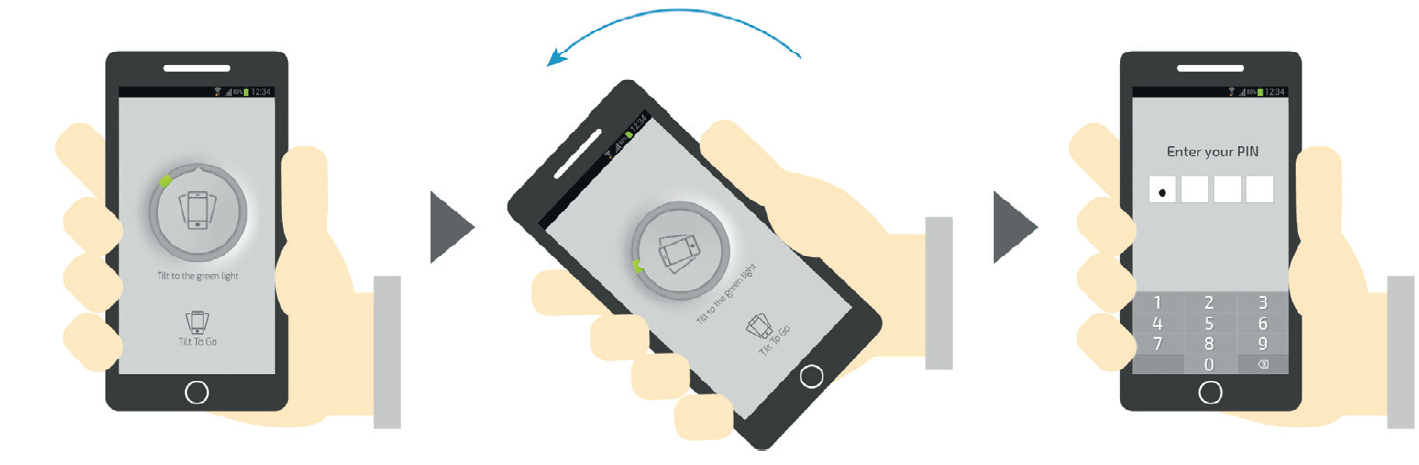
\includegraphics[width=.8\linewidth]{Images/StateOfArt/CAPPCHA}
     \caption{\footnotesize{CAPPCHA and PIN authentication\cite{CAPPCHA}.}}\label{soa:CAPPCHA}
\end{figure}
}
\descItem{Invisible CAPPCHA}
{It will be described in details in \myref{Chapter}{chapter:InvisibleCAPPCHA}.}
\end{itemize}

\section{CAPTCHA security}\label{soa:security_CAPTCHAs}
The process used to break many traditional CAPTCHAs, based on text or images, is usually organized into the following phases\cite{CAPTCHA_attack_process}:
\begin{enumerate}
\descItem{Pre-processing phase}
{in this phase, several techniques are applied to remove background, to separate foreground from the background, to delete noise and to remove some particular pattern (e.g. Canny Detection and Scale-Invariant Feature Transform (SIFT) application).
}
\descItem{Attack phase}
{the following techniques are usually applied:
\begin{itemize}
\descItem{\textit{Object recognition attacks}}
{The most used techniques are pattern matching (e.g. shape context matching, correlation algorithm), OCR recognition, SIFT and machine learning. They are usually applied after the segmentation of the image with several methods (e.g. vertical histogram, color filling, snake segmentation and JSEG).}
\descItem{\textit{Random Guess Attacks}}
{The attacker's program tries to break the CAPTCHA scheme by guessing the correct answer. This attack is effective on CAPTCHAs with few number of different challenges.}
\descItem{\textit{Human Solver Relay Attacks}}
{The bot forwards the CAPTCHA challenge to a remote human worker that will solve it if the previous phases don't produce good results. This technique is usually used also to solve other types of CAPTCHAs.}
\end{itemize}
}
\end{enumerate}
Many CAPTCHA schemes have still several issues:
\begin{itemize}
\descItem{Session issue}
{Some types of CAPTCHAs have a big issue because they don't destroy the session, after a correct answer is inserted by the user\cite{text_audio}.\\
Hence, the hacker can crack the next accesses using the same session id with the related solution of the challenge, after connecting to the web page of CAPTCHA. In this way the attacker can make hundreds of requests before the session expires and the previous operation must be computed again.}
\descItem{Resilience to both automated and human solver relay attacks}
{Many CAPTCHA schemes are designed to be robust against a possible AI attack but the new generation of CAPTCHAs involves the use of remote bot or human solver. Traditional CAPTCHA schemes are vulnerable to this type of attacks.\\
Sensor-based CAPTCHAs are often vulnerable to relay attacks. An exception is the \textit{Invisible CAPPCHA}, that will be analysed in \myref{Chapter}{chapter:InvisibleCAPPCHA}.
}
\descItem{Limited number of challenges}
{An issue of sensor-based CAPTCHA schemes is the limited number of challenges because the design of many usable gestures is very hard. This problem could be solved
relying on trusted hardware.}
\descItem{Trade-off between Friction-heavy and Frictionless CAPTCHAs}
{A trade-off between usability and security aspects is always considered analysing CAPTCHA schemes. This condition is exacerbated in behavioural and sensor-based CAPTCHAs.}
\descItem{User's privacy}
{Sensor-based and behavioural CAPTCHAs usually send useful information to a remote server that analyses it to establish if the user was a human or a bot. If an hacker attacks the server side of this application, he can access users' private data.\\
In some CAPTCHAs, the information is evaluated on the client side by a trusted hardware and the server receives only the results of the analysis. In this case, we need to be sure that trusted hardware is secure enough to guarantee privacy of user's information.
}
\descItem{Compatibility with different devices}
{Many CAPTCHA schemes, e.g. behavioural ones, use specific forms factors but a good challenge should be compatible with different factors.}
\end{itemize}

\begin{sidewaystable}
\centering \footnotesize
\renewcommand*\arraystretch{1.3}
\begin{tabular}{ccll}
\toprule
\multicolumn{1}{c}{\textbf{Type}} & \multicolumn{1}{c}{\textbf{Scheme}} & \multicolumn{1}{c}{\textbf{Usability issues}} & \multicolumn{1}{c}{\textbf{Security}}\\
\midrule
%Audio row
\multirow{3}{*}{\textbf{\textit{Audio}}} & {\textit{Audio reCAPTCHA}} & {Issues of recognition:} & {It's vulnerable to:}\\
&&{\itemCell{Knowledge of English dictionary by the user.}}&{\itemCell{ASR programs.}}\\
&&{\itemCell{Some character sounds very similar to others.}}&{\itemCell{Deep Learning and ML techniques.}}\\
\midrule
\multirow{2}{*}{\textbf{\textit{Game}}} & {\textit{Dynamic Cognitive}} & {Comprehension of rules.} & {Vulnerable to Stream Relay Attack}\\
& {\textit{Game (DCG)}} &&\\
\midrule
\multirow{5}{*}{\textbf{\textit{Image}}} & {\textit{Click-based}} & {Difficulty in identification of images caused by:} & {Vulnerable to:}\\
& {\textit{Drag \& Drop-based}} & {\itemCell{Blur of images.}} & {\itemCell{Segmentation techniques}}\\
& {\textit{Sliding-based}} & {\itemCell{Low vision condition.}} & {\itemCell{Deep Learning and ML techniques}}\\
& {\textit{Selection-based}} && {OCR techniques}\\
& {\textit{Interactive-based}} &&\\
\midrule
%Math row
\multirow{3}{*}{\textbf{\textit{Math}}} & {\textit{Arithmetic}} & {It requires basic or advanced} & {Vulnerable to:}\\
{} & {\textit{QRBGS}} & {math knowledge.} & {\itemCell{OCR techniques}}\\
&&&{\itemCell{Side-channel attacks}}\\
\midrule
\multirow{2}{*}{\textbf{\textit{Slider}}} & {Taobao.com} & {Simple and intuitive interaction} & {Simple bypassed by Javascript code}\\
& {TheyMakeApps.com} & {} & {and pupeeteer}\\
\midrule
\multirow{5}{*}{\textbf{\textit{Text}}} & {\textit{2D}} & {Many problems have to be solved by user:} & {It can be identified by:}\\
&{\textit{3D}}&{\itemCell{Multiple fonts}}&{\itemCell{OCR technique}}\\
&&{\itemCell{Font size}}&{\itemCell{Segmentation techniques}}\\
&&{\itemCell{Blurred Letters}}&{\itemCell{Deep Learning and ML techniques}}\\
&&{\itemCell{Wave Motion}}&\\
\midrule
{\textbf{\textit{Video}}} & {\textit{Motion CAPTCHA}} & {Heavy file to be downloaded} & {}\\
\bottomrule
\end{tabular}
\caption{\footnotesize{Survey of main types of traditional CAPTCHAs\cite{survey_CAPTCHA}.}}
\label{soa:traditional_table}
\end{sidewaystable}

\begin{comment}
\begin{sidewaystable}
\centering \footnotesize
\renewcommand*\arraystretch{1.3}
\begin{tabular}{ccll}
\toprule
\multicolumn{1}{c}{\textbf{Alternative Type}} & \multicolumn{1}{c}{\textbf{Name of implementation}} & \multicolumn{1}{c}{\textbf{Usability issues}} & \multicolumn{1}{c}{\textbf{Security}}\\
\midrule
\textit{} & {} & {}\\
\bottomrule
\end{tabular}
\caption{\footnotesize{Survey of main types of alternatives of CAPTCHAs\cite{survey_CAPTCHA}.}}
\label{soa:modern_table}
\end{sidewaystable}
\end{comment}
\chapter{Side-channel attacks}\label{chapter:SideCH}
A side-channel attack is an attack in which the malicious user exploits a side-information of transmitted encrypted data, to give access to user private data. 
This type of extra information is usually: timing information, power consumption, electromagnetic radiations, sound and so on.\\
The first types of side-channel attacks requires the physical access to the victim's device. Nowadays, side-channel attacks are evolved and can be conducted by remote hackers using malicious code (e.g. cache-timing attacks, DRAM row buffer attacks), even exploiting information from sensors on mobile devices\cite{side_classification}.\\
Side-channel attacks can be classified as:
\begin{itemize}
\descItem{active}{the hacker influences the behaviour of the victim's device}
\descItem{passive}{the attacker only analyses the leaking information}
\end{itemize}
Another categorization can be the following one:
\begin{itemize}
\item{Local attacks}
\item{Vicinity attacks}
\item{Remote attacks}
\end{itemize}
In the following sections there is a survey of the most popular attacks, organized with respect to the previous classifications (see \myref{Table}{sc:review}). 
The main sensors, that are usually exploited by an hacker to obtain side-channel information on mobile devices, are\cite{side_attacks}:
\begin{itemize}
\item{Location sensors (e.g. GPS, proximity)}
\item{Motion sensors (e.g. accelerometer, gyroscope, magnetometer)}
\item{Environmental sensors (e.g. for ambient light, temperature, barometer)}
\item{Biometric sensors for wearable devices (e.g. heart rate sensor, ECG)}
\item{Audio sensors (microphone)}
\item{Video sensors (camera)}
\end{itemize}

\begin{table}[h]
\centering \footnotesize
\renewcommand*\arraystretch{1.3}
\begin{tabular}{rlll}
\toprule
{} & \multicolumn{1}{c}{\textbf{Local}} & \multicolumn{1}{c}{\textbf{Vicinity}} & \multicolumn{1}{c}{\textbf{Remote}}\\
\midrule
\verticalCell{9}{\textbf{Passive}} & {Power Analysis} & {Network Traffic Analysis} & {Linux-inherited procfs Leaks}\\
& {Electromagnetic Analysis Attacks} &  {USB Power Analysis} & {Data-Usage Statistics}\\
& {Differential Computation Analysis} & {Wi-Fi Signal Monitoring} & {Page Deduplication}\\
& {Smudge Attacks} &  & {Microarchitectural Attacks}\\
& {Shoulder Surfing and Reflections} &  & {Sensor-based Keyloggers}\\
& {Hand/Device Movements} &  & {Fingerprinting Devices/Users}\\
&  &  & {Location Inference}\\
&  &  & {Speech Recognition}\\
&  &  & {Soundcomber}\\
\midrule
\verticalCell{6}{\textbf{Active}} & {Clock/Power Glitching} &\\
& {Electromagnetic Fault Injection (EMFI)} & {Network Traffic Analysis} & {Rowhammer}\\
& {Laser/Optical Faults} &  & \\
& {Temperature Variation} &  & \\
& {Differential Computation Analysis} &  & \\
& {NAND Mirroring} &  & \\
\bottomrule
\end{tabular}
\caption{\footnotesize{Survey of the most popular side-channel attacks\cite{side_classification}.}}
\label{sc:review}
\end{table}

\section{Local side-channel attacks}
The attacker needs to get the target device or to be very near to it. In many cases the hacker physically needs to manipulate the the device or to obtain access to the chip.\\\\
\textbf{Passive attacks}\\
The following attacks are used to break cryptographic system implementations:
\begin{itemize}
\descItem{\textit{Power Analysis}}
{this type of attacks are based on the analysis of the power variations in transistors. There exist several attacks\cite{intro_DPA}:
\begin{itemize}
\descItem{\textit{Simple Power Analysis (SPA)}}
{the attacker analyses the power consumption of the system, that depends on the microprocessor used. This analysis can be useful to understand which operations are performed by different implementations of cryptographic algorithm (e.g. RSA, DES).}
\descItem{\textit{Differential Power Analysis (DPA)}}
{these attacks collect data and then makes statistical analysis and error correction techniques from data to extract information correlated to secret keys.}
\descItem{\textit{High Order DPA (HO-DPA)}}
{While DPA obtains information across a single event, HO-DPA correlates between multiple cryptographic sub-operations.}
\end{itemize}}
\descItem{\textit{Electromagnetic Analysis Attacks}}
{the attacker can analyse indirectly the power consumption by accessing electromagnetic. This type of attacks depends on the used instruments (e.g. EM probes) and on the analysed location of the chip, affecting the signal-to-noise ratio.}
\descItem{\textit{Differential Computation Analysis}}
{the attacker tries to exploit white-box cryptographic implementations. In this model the attacker, even if he has access to code, can't extract the secret key. The attacker needs to have full control over the target device and the execution environment. Then using binary instruments, he can control the intermediate state or memory operations (e.g. reading/writing operations)\cite{side_DCA}.}
\descItem{\textit{Smudge Attacks}}
{the attacker can exploit fingerprints and smudges on the screen of mobile devices to evaluate the user's input.}
\descItem{\textit{Shoulder Surfing and Reflections}}
{the attacker can exploit the lightness of the device display and obtain the user's activity by its reflection on sunglasses or tea pods.}
\descItem{\textit{Hand/Device Movements}}
{the attacker exploits the user's movements of fingers and hand to understand the interaction of the victim with the device.}
\end{itemize}
\textbf{Active attacks}\\
The following attacks require that the hacker physically gets the device for a while:
\begin{itemize}
\descItem{\textit{Clock/Power Glitching}}
{in the past the attacker can fault inject on embedded devices by exploiting variations of the clock signal, (e.g. overclocking). To do it, he needs to use an external clock source.}
\descItem{\textit{Electromagnetic Fault Injection (EMFI)}}
{the attacker uses short (e.g. nanoseconds), high-energy electromagnetic pulses to change the state of memory cells. This attack allows to target specific regions of a microchip by locating the EM probe (e.g. on the instruction memory, the data memory, or CPU registers).}
\descItem{\textit{Laser/Optical Faults}}
{the attacker needs to decapsulate the chip to obtain access to it and, using a laser beam, it change the state of a transistor (e.g. changing bit value of a memory cell).}
\descItem{\textit{Temperature Variation}}
{the attacker can change the temperature in which the target device, causing malfunctioning of the hardware. Temperature higher than the maximum one, supported by hardware, causes faults in memory cells. Temperature too lower changes the speed, for which the content of the RAM disappear, after turning the device off.}
\descItem{\textit{Differential Computation Analysis}}
{the attacker needs to have full control of the white-box environment, manipulating intermediate values in the system computation.}
\descItem{\textit{NAND Mirroring}}
{the attacker exploits the duplication of the data, usually used to recover data after faults, to restore a previous system state. The hacker can force the reset of the state as demonstrated by Skorobogatov for the Apple case\cite{side_apple}.}
\end{itemize}


\section{Vicinity side-channel attacks}
The attacker needs to wiretap or eavesdrop the network communication of the victim or to be in the neighbourhood of the target.\\\\
\textbf{Passive attacks}
\begin{itemize}
\descItem{\textit{Network Traffic Analysis}}
{the attacker can exploit meta data, related to the encrypted data, transmitted over the network. This information gives access to sensitive information about the traffic.\\
For example a Web-application works between two parties: the client and the server. For this reason the communication channel is usually encrypted and the requests made by the user work through the \textit{HTTPS} protocol.\\
This solution isn't enough to prevent an attacker to exploit reserved data because each web page has a distinct size, loads resources of different sizes. Hence the attacker can fingerprint the page even if HTTPS protocol is used.\\
Another cause of these attack on Web-services is given by the trend of Web to work on Stateful Protocols, providing better performance to the client by keeping track of the connection information. TCP session for example works on Stateful Protocol because both systems maintain information about the session itself during its life\cite{side_leaks}.\\}
\descItem{\textit{USB Power Analysis}}
{the attacker can modify USB charging stations for mobile devices to obtain analysis about power consumption and related sensitive information.}
\descItem{\textit{Wi-Fi Signal Monitoring}}
{Wi-Fi devices continuously monitor the wireless channel (channel state information (CSI))
to transmit data. Any environmental variation (e.g. finger motion) affects Wireless signals, generating unique pattern in CSI series. For example the attacker can exploit these variations to unlock patterns on smartphones\cite{side_CSI}.}
\end{itemize}
\textbf{Active attacks}
\begin{itemize}
\descItem{Network Traffic Analysis}
{the attacker, after obtaining information about transmitted packets, can interfere the traffic (e.g. delay of packets).}
\end{itemize}


\section{Remote side-channel attacks}
These attacks are software-only based and they depend on the installation of the malicious code on the target device. 
\textbf{Passive attacks}
\begin{itemize}
\descItem{\textit{Linux-inherited procfs Leaks}}
{the attacker can obtain a large amount of information for each process running on Linux File System, by looking to the content of the files, reported in \myref{Table}{sc:proc}.
\begin{table}[h]
\centering \footnotesize
\renewcommand*\arraystretch{1.3}
\begin{tabular}{rl}
\toprule
\multicolumn{1}{c}{\textbf{File path}} & \multicolumn{1}{c}{\textbf{Information}}\\
\midrule
{\textbf{\textit{/proc/[pid]/statm}}} & {Virtual and physical memory sizes of process with identifier \textit{[pid]}}\\
{\textbf{\textit{/proc/[pid]/stat}}} & {CPU utilization times of process with identifier \textit{[pid]}}\\
{\textbf{\textit{/proc/[pid]/status}}} & {Number of context switches of process with identifier \textit{[pid]}}\\
{\textbf{\textit{/proc/interrupts}}} & {Interrupt counters}\\
{\textbf{\textit{/proc/stat}}} & {Context switches}\\
\bottomrule
\end{tabular}
\caption{\footnotesize{Survey of the most popular side-channel attacks\cite{side_classification}.}}
\label{sc:proc}
\end{table}
}
\descItem{\textit{Data-Usage Statistics}}
{the attacker can access to information about incoming and outgoing network traffic for each application without any permission.}
\descItem{\textit{Page Deduplication}}
{To reduce the overall memory footprint of a system, some operating systems perform deduplication, searching for identical pages within the physical memory and merge them even across different processes. When a process tries to write on a deduplicated page, a copy-on-write fault occurs and the process gets its own copy of this memory region again.}
\descItem{\textit{Microarchitectural Attacks}}
{By measuring execution times and memory accesses, the attacker can obtain sensitive information from processes running in parallel on the same device. This type of information can be evaluated from CPU caches, that are a big source of information leaks.}
\descItem{\textit{Sensor-based Keyloggers}}
{in mobile devices, the attacker can exploit information from equipped sensors with any permission. The user's interaction with the device can be evaluated by analysing information from sensors.}
\descItem{\textit{Fingerprinting Devices/Users}}
{the attacker can obtain identity of the device and the user and fingerprint by exploiting hardware issues and cookies.}
\descItem{\textit{Location Inference}}
{the attacker can obtain user's location without using GPS sensor, that requires permission to be accessed. For example, the accelerometer and the gyroscope can be used to infer car driving routes.}
\descItem{\textit{Speech Recognition}}
{the access to the microphone is protected by permissions. The attacker can also exploit gyroscope to obtain information about human speech near to the device.}
\descItem{\textit{Soundcomber}}
{the attacker can obtain sensitive information (e.g. credit card numbers) on automated menu services of phones after he obtains permission of access to the microphone.}
\end{itemize}
\textbf{Active attacks}
\begin{itemize}
\descItem{\textit{Rowhammer}}
{the attacker can induce hardware faults by frequent accesses to main memory. This happens because nowadays the size of DRAM cells decreases to increase the density of memory cells in DRAM causing electromagnetic coupling effects between cells.}
\end{itemize}

\chapter{Invisible CAPPCHA}\label{chapter:InvisibleCAPPCHA}
The \textit{Invisible CAPPCHA} is an evolution of CAPPCHA, in terms of usability\cite{Invisible_CAPPCHA}. The main difference with respect to CAPPCHA is that the challenge is not explicitly submitted to the user but it is embedded in the PIN authentication phase leveraging a side channel. Invisible CAPPCHA works only on smartphones as its ancestor but it's very important to understand how data, obtained by the sensors, could be leveraged during the authentication phase.\\
Invisible CAPPCHA is a method developed in 2018 and based on motion side-channel of mobile devices and it's very effective as support to Password-based authentication methods. The main steps, followed by this CAPTCHA, are:
\begin{enumerate}
\descItem{Motion detection}{in this phase the micro-movements of the device, generated by the interaction of the user with the touch-screen, are evaluated by the \textit{Secure Element} (\textit{SE})}
\descItem{Communication between Client and Server}{in this phase the credentials are shared with the remote Service Provider}
\end{enumerate}
The following sections will analyse this steps highlighting some peculiarities of Invisible CAPPCHA that will be used or modified to develop AcCAPPCHA, a CAPTCHA based on microphone sensors.

\section{Motion detection}
In this first phase, Invisible CAPPCHA exploits the accelerometer of the mobile device. It detects the acceleration over the three axis in g-force units, as a sequence of vectors over time:
$$\{ A_i\}_{i=1}^{n} = \{ (a_1^x, a_1^y, a_1^z), ..., (a_n^x, a_n^y, a_n^z)\}$$
This type of side-channel information from embedded accelerometer has been exploited in different attacks for the single and double tap detection. These attacks analyse the accelerations over the z-axis by comparing them to some thresholds and some timing conditions.\\
In Invisible CAPPCHA, the side-channel information is stored on the memory of the mobile device. Depending on the device, a smartphone built-in vibration can be generated along Z axis or along more than one axis (see \myref{Figure}{inv:vibration}). On the contrary a finger tap event is defined by strong accelerations on Z-axis but also similar one to the other (see \myref{Figure}{inv:tap}).\\
In Invisible CAPPCHA, the difference between built-in vibration and tap acceleration is evaluated by a simple algorithm. It relies on negative and positive peaks, that are detected by comparing acceleration along Z axis with predefined thresholds. The differences between the tap accelerations and the vibrations is the main characteristic that guarantees user's tap cannot be simulated by a bot using the vibration motors.\\
Another important requirement, to prevent a bot attack, is that Invisible CAPPCHA uses a Secure Element that embedded the accelerometer of the device. In this way malicious code can't access to the sensor. Nowadays there exists a smart card, called SIMSense, that already integrates motion sensor and embeds it in a Secure Element.\\
\begin{figure}[h]
     \centering
     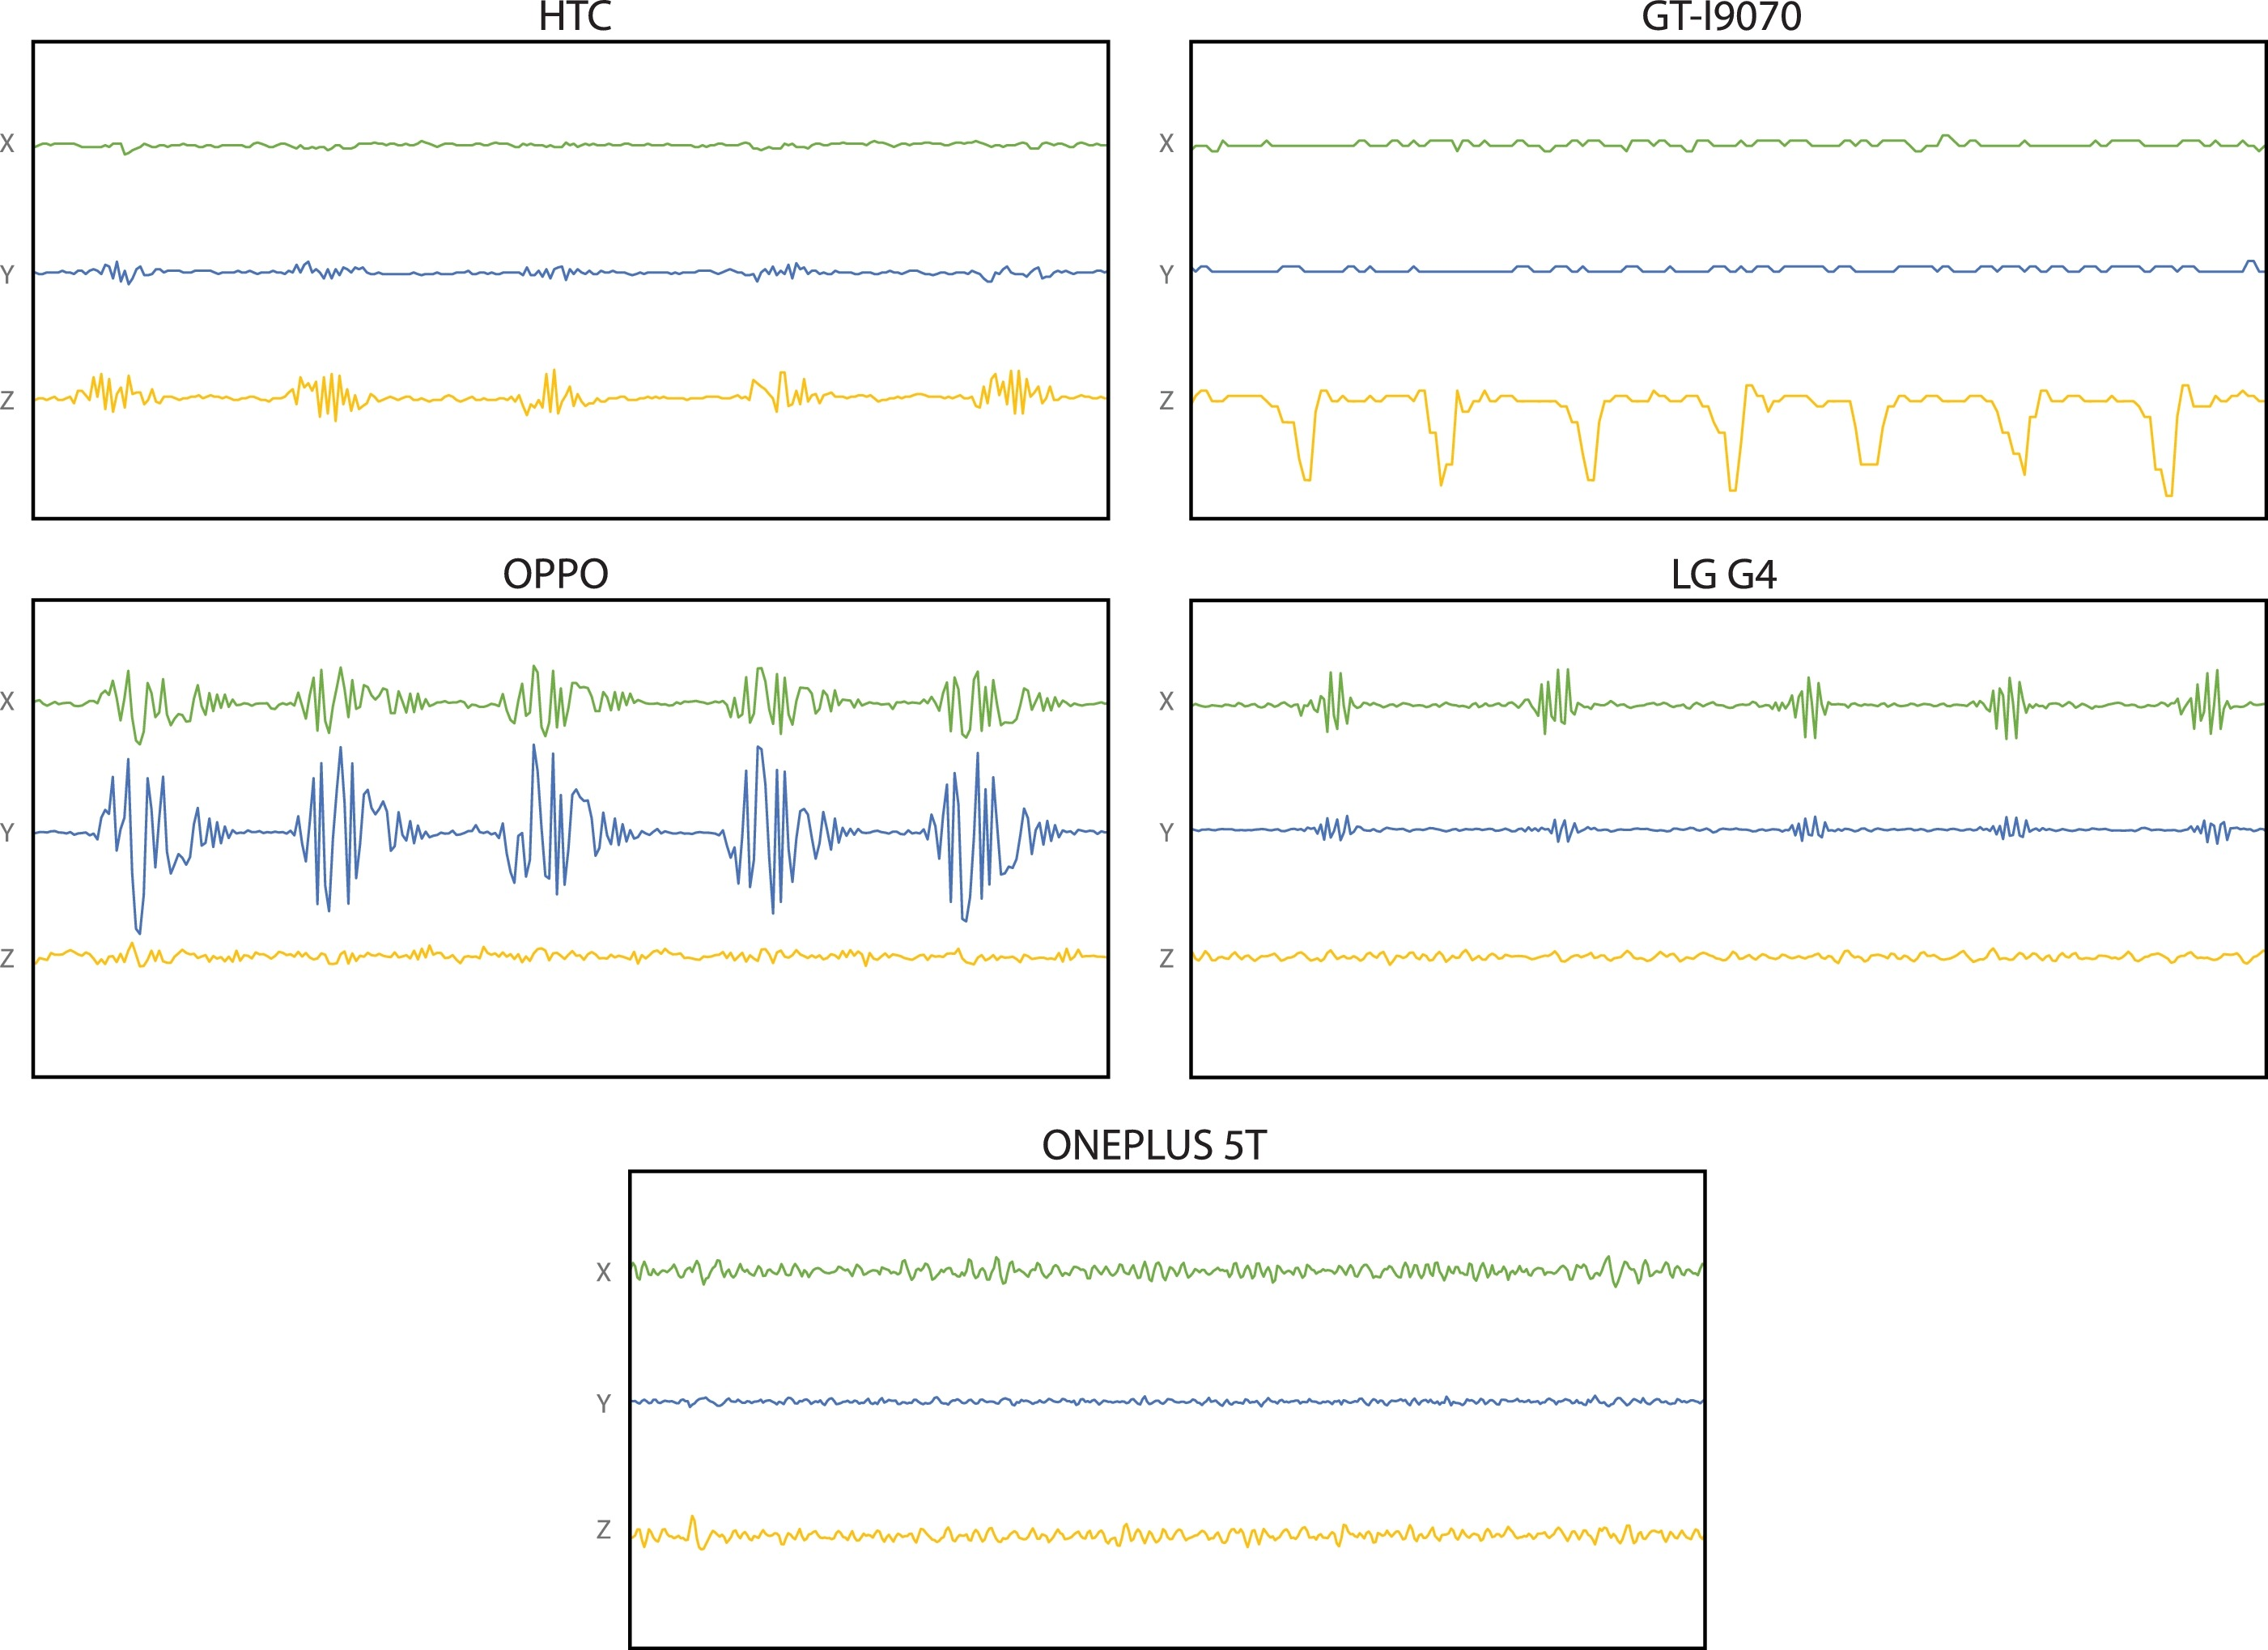
\includegraphics[width=.8\linewidth]{Images/InvisibleCAPPCHA/vibration}
     \caption{\footnotesize{Example of accelerations caused by smartphone built-in vibration.}}\label{inv:vibration}
\end{figure}
\begin{figure}[h]
     \centering
     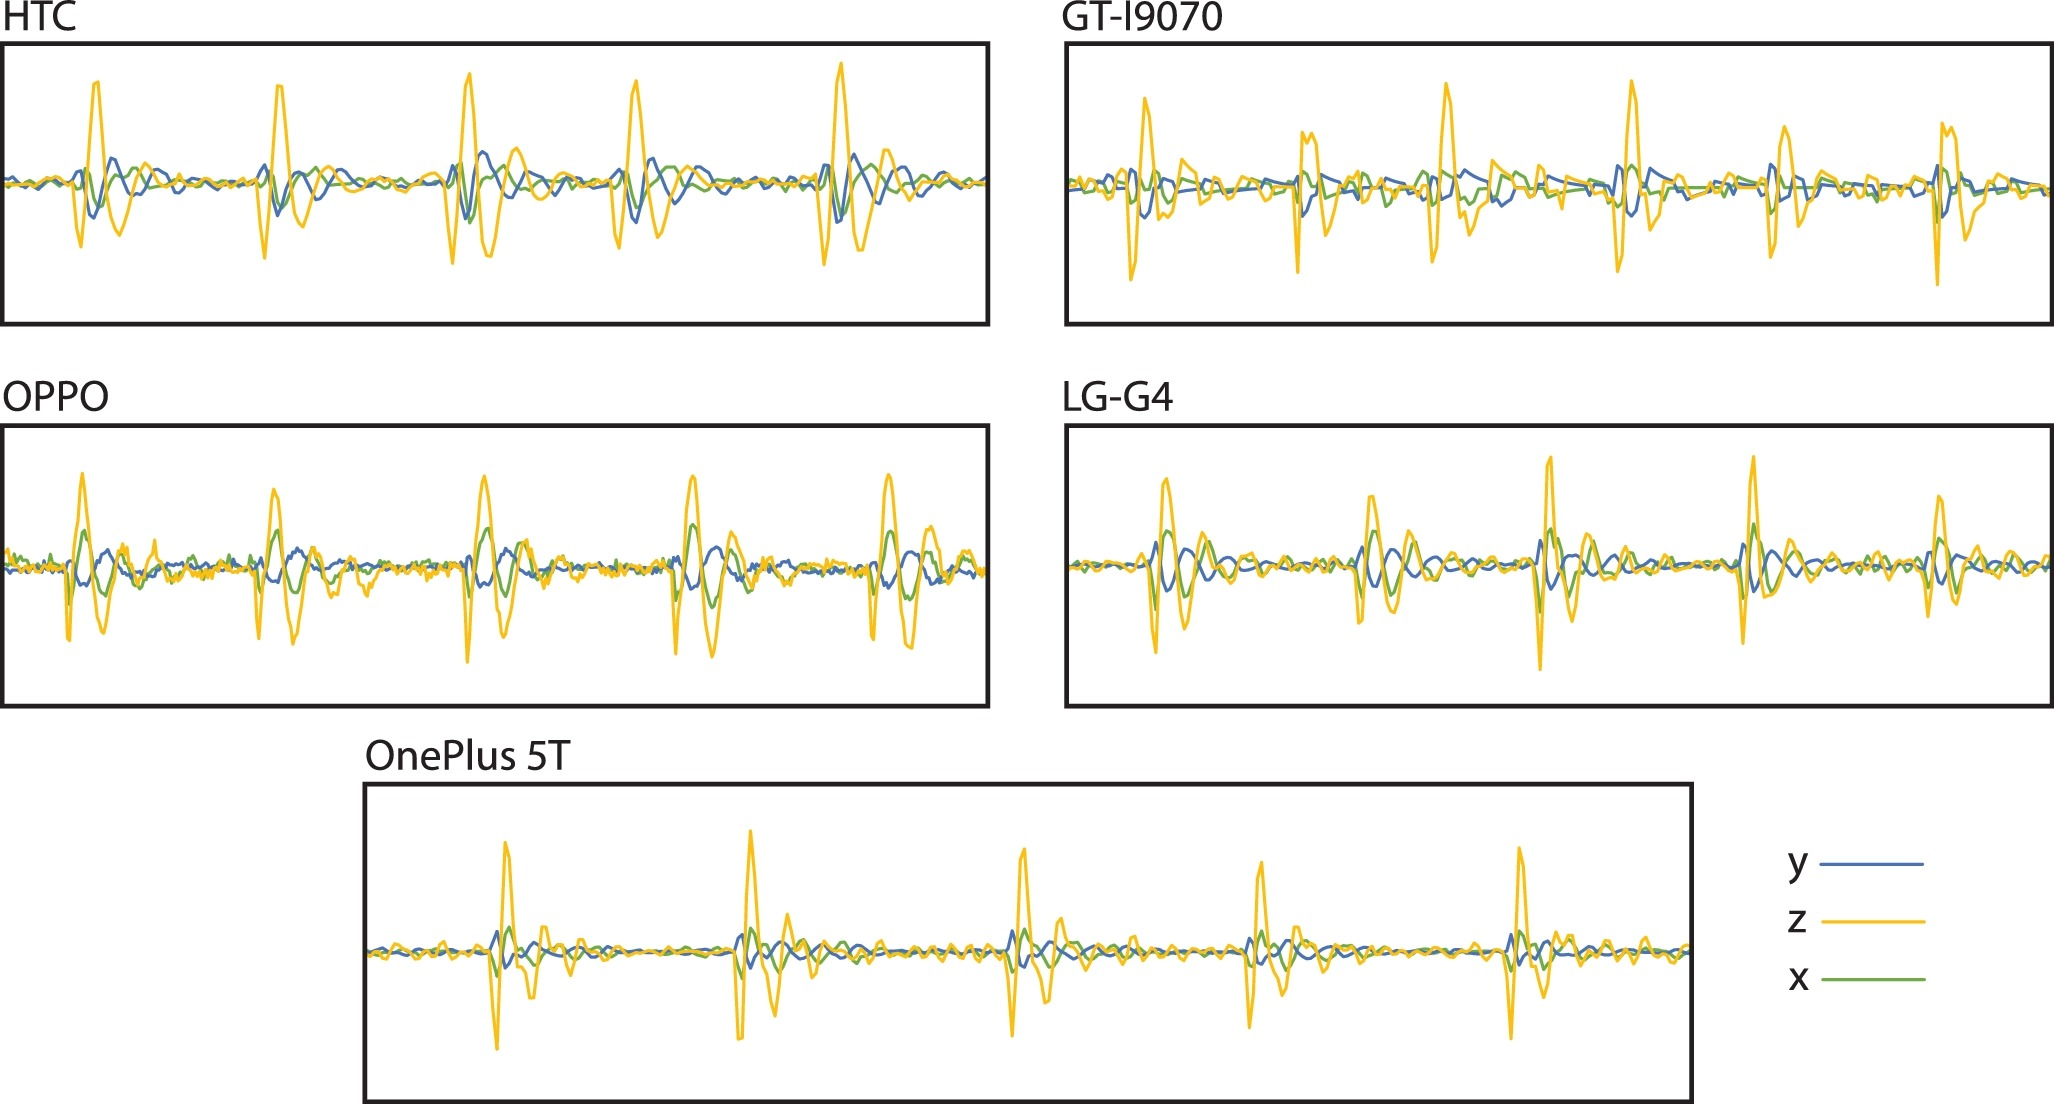
\includegraphics[width=.8\linewidth]{Images/InvisibleCAPPCHA/tap}
     \caption{\footnotesize{Example of accelerations caused by finger tap detection.}}\label{inv:tap}
\end{figure}


\section{Communication between Client and Server}\label{inv:communication}
When the user fills a form or provides other information to a cloud application/service, the Secure Element checks if a micro-movement is measured when a user tap is detect. If this happens the input inserted by user is considered valid, or rather generated by a human, otherwise the algorithm tells that the input was generated by a bot.\\
An extra message, that tells if the task was performed by a user or not, is sent to the server side. The integrity of this message is guaranteed by the Secure Element, that can be equipped with a digital signature. The identity of the device can be associated to the message sent and then it can be checked and verified. The Secure Element signs the verification message through ECDSA.

\subsection{Elliptic Curve Digital Signature Algorithm (ECDSA)}
The elliptic cryptography works similarly to RSA but it uses smaller keys. The signature algorithm with elliptic curves is divided in two phases, like the one based on RSA. Considering two users, Alice and Bob, ECDSA phases are explained in the following lines:
\begin{itemize}
\descItem{Sign generation}
{If Alice wants to send a message, protected with digital sign, to Bob, they need to share the following parameters \textit{(curve, G, n)}: \textit{curve} is the equation of an elliptic curve, \textit{G} is the base point of prime order on the curve and \textit{n} is the multiplicative order of \textit{G} for which $n\; x\; G = O$ ($x$ is the scalar multiplication of a point of the curve).
Alice generates a private key $d_A$ in the range $[1, n-1]$ and a public key $Q_A=d_A\; x\; G$. Alice needs to perform \myref{Algorithm}{inv:ECDSA_sign} to sign a message $m$.
\begin{algorithm}[h]
\DontPrintSemicolon\footnotesize
\KwIn {$\mathtt{m}$= message to be signed}
\KwOut {$\mathtt{(r,s)}$= digital sign}
\BlankLine
$e\gets HASH(m)\;$where \textit{HASH} is an hash function (e.g. SHA-2)\;
\BlankLine
$z \gets$ string composed by the $L_n$ most left bits\;
$\;\;\;\;\;\;\;$where $L_n$ is the bit length of the group of order $n$\;
$r\gets 0$\;
$s\gets 0$\;
\BlankLine
\While{$r=0\;mod\;n$ or $r=0\;mod\;n$}{
	\BlankLine
	$k\gets RANDOM([1,n-1])$\;
	\BlankLine
	$(x_1, y_1)=k\;x\;G$ of the elliptic curve\;
	\BlankLine
	$r\gets x_1\; mod\; n$\;
	\BlankLine
	{$s\gets k^{-1}(z+rd_{A})\; mod\; n$}
	\BlankLine
}
\caption{Sign generation.}\label{inv:ECDSA_sign}
\end{algorithm}
}
\descItem{Sign verification}
{Bob wants to verify the digital signature sent by Alice. To do it, he needs to apply in order \myref{Algorithm}{inv:ECDSA_key_verify} and \textbf{\ref{inv:ECDSA_verify}}.\\
\begin{algorithm}[h]
\DontPrintSemicolon\footnotesize
\KwIn {$\mathtt{Q_A}$= public key to be verified}
\KwOut {$\mathtt{check}$= true if public key is correct}
\BlankLine
$\mathtt{check}\gets true$\;
\BlankLine
$\setminus\setminus$Valid coordinates\;
\If{$Q_A=O$}
{	
$\mathtt{check}\gets false$\;
}
\BlankLine
$\setminus\setminus$Element of the curve\;
\If{$Q_A\;\in$ curve}
{	
$\mathtt{check}\gets false$\;
}
\BlankLine
$\setminus\setminus$Correctness of order\;
\If{not $n\;x\;Q_A=O$}
{	
$\mathtt{check}\gets false$\;
}
\caption{Verification that public key is on the elliptic curve.}\label{inv:ECDSA_key_verify}
\end{algorithm}
\begin{algorithm}[h]
\DontPrintSemicolon\footnotesize
\KwIn {$\mathtt{(r,s,m)}$= digital sign and message}
\KwOut {$\mathtt{m}$= message to be signed}
\BlankLine
$e\gets HASH(m)\;$where \textit{HASH} is an hash function (e.g. SHA-2)\;
\BlankLine
$z \gets$ string composed by the $L_n$ most left bits\;
where $L_n$ is the bit length of the group of order $n$\;
\BlankLine
\If{not $r\;\in [1, n-1]$ or not $s\;\in [1, n-1]$}
{*Invalid sign*}
$e\gets HASH(m)\;$\;
\BlankLine$z \gets$ string composed by the $L_n$ most left bits\;
$w=s^{-1}\; mod\; n$\;
\BlankLine
$u_1 =zw\; mod\; n$\;
$u_2 =rw\; mod\; n$\;
$(x_1, y_1)=u_1\; x\; G\;+\; u_2\; x\; Q_{A}$ of the elliptic curve\;
\BlankLine
\If{$r\equiv x_1\; (mod\; n)$}
{*Verified sign*}
\Else{*Not accepted sign*}
\BlankLine
\caption{Sign verification.}\label{inv:ECDSA_verify}
\end{algorithm}
}
\end{itemize}
In Invisible CAPPCHA the message \textit{m} is bitwise concatenated with a signed unique value, the nonce \textit{n}, and then the signature is computed on their concatenation, $m||n$. Hence the signed message sent to the server is $(r, s, m, n)$.

\section{Security analysis}
After the verification of the signature, the communication must be also encrypted to ensure integrity and authenticity of exchanged messages.\\
The Secure Element can be accessed only through PIN authentication of the off-card communication party. If the malicious code has enough privileges to access Secure Element, some popular attacks can't be performed by an attacker.\\

\subsection{Strength against popular attacks}\label{inv:attacks}
The most popular attacks, that have been analysed, are\cite{Invisible_CAPPCHA}:
\begin{itemize}
\descItem{Replay attack}
{Because the message is signed together with a nonce, an attacker can't easily use a message already sent by a client to the server. In fact, the server checks if a nonce was already used by the client and if so, the server refuse the message sent by the attacker.
}
\descItem{Reverse engineering attack}
{Even if the attacker can de-obfuscate the code of the application running on the browser, he can access to reserved data on the server only if the verification message for human interaction was correctly signed by the Secure Element. Hence this type of attack can't be performed.}
\descItem{Human-solver relay attack}
{The Invisible CAPPCHA is strong to this type of attack because it doesn't require any additional task to be sent to a remote human solver, as in standard CAPTCHAs.}
\descItem{Brute force and password replay attacks}
{Invisible CAPPCHA can be used to validate every input before it is considered as a possible attempt for a password. If the password was inserted by a malware or was wrong, the number of attempts decreases. Hence this approach prevents a brute force attack. This also prevents the access to the Secure Element by the attacker in replay attacks.
}
\descItem{Denial Of Service (DOS)}
{If a malware tried more than the maximum amount of attempts of passwords it could do a Denial Of Service (DOS) of the Secure Element. To prevent this attack, the Secure Element can block access to itself if three invalid passwords are inserted by a human or if an invalid password is inserted by a bot.}
\end{itemize}
\chapter{AcCAPPCHA}\label{chapter:AcCAPPCHA}
AcCAPPCHA is a verification method that works like a key-logger. This type of programs is usually malicious and intended to be used by an attacker to acquire information about the user's activity. This application analyses the sequence of keys inserted by exploiting side-channel information. Its implementation depends on the party, that the hacker wants to attack\cite{keylogging}, and that could be:
\begin{itemize}
\descItem{The user}
{these attacks are based on the exploitation of physical information related to the typing state. For example, they can use electroencephalography (EEG), motion of the wrist in the smartwatches, video with keyboard line-of-sight and WiFi signal distortion.}
\descItem{The keyboard}
{these attacks are based on analysis of signals coming from the keyboard. For example, acoustic emanations can be exploited by using external physical sensors.}
\descItem{The host}
{these attacks are based on the physical access of the attacker to the victim machine. For example, the process footprint, the CPU load and other micro-architectural analysis can be exploited in this attacks.}
\descItem{The network}
{these attacks exploit the packets exchanged in the client-server communication. For example, a network packet can be related to a keystroke revealing the key press time of the victim and the payload size of the server response.}
\end{itemize}
Analysing the previous key-logger based on side-channel information, attacks mentioned in \myref{Chapter}{chapter:SideCH} and the structure of Invisible CAPPCHA in Section \myref{Section}{chapter:InvisibleCAPPCHA}, I design this new implementation of CAPTCHA. It exploits acoustic side-channel of the microphone to implement a particular type of keylogger that ensures that the Authentication phase would be performed by a human user.\\
The whole implementation was created using \texttt{Python} language. The structure and the behaviour of AcCAPPCHA are similar to the ones proposed in Invisible CAPPCHA because they are both based on the evaluation of signal, detected by some sensor (motion sensors for Invisible CAPPCHA and microphone for AcCAPPCHA). With respect to Invisible CAPPCHA the program can perform also a classification of the audio signal using neural networks. The two phases of the verification are:
\begin{itemize}
\item{Evaluation of the user's activity}
\item{Communication with the remote service}
\end{itemize}
In the second phase, the username and the password of the user will be signed through ECDSA and sent by client to the authentication service if and only if the insertion was performed by a human.

\section{Evaluation of the user's activity}\label{AcCAPPCHA:user_activity}
AcCAPPCHA records two audio signals: the first one created during the insertion of the password by the user and the second one created before this activity for the noise evaluation. The first signal is The second signal is exploited to evaluate a noise threshold useful for the computation of amplitude peaks in the first audio.
During the insertion of the password, the instants of the time when each character was typed by the user are stored. 

\subsection{Time correspondence}\label{AcCAPPCHA:time_correspondence}
Before asking the user to insert the password, the program records an audio file of 1 second, called \texttt{noise signal}, from the built-in microphone of the laptop. The remaining verification procedure is performed by two threads simultaneously, during password insertion. The first one is continuously waiting for the insertion of a character of the password by the user until he types CARRIAGE RETURN\textit{'\r'}).\\
Immediately after a key is pressed, the time instant of this action, related to the Epoch of the PC, is stored. The sequence of time instants stored by the thread is called $x=(x_0, ..., x_{|password|-1})$. The second thread records an audio signal, called \texttt{user activity}, using the same hardware previously mentioned. This task begins its activity before the request of the password to the user and would end after the moment in which the first thread detects a CARRIAGE RETURN. Then the application removes the last 200 ms of this audio signal to be sure that the \textit{CARRIAGE RETURN} peak isn't included in recorded audio file.\\
From now on, the application has all it needs to understand if the user is a human or not. In fact the verification is performed by looking if there exists a sequence of time instants of the peaks in the signal recorded in parallel to the insertion of the password and the time instants manually stored for each character.\\
In particular \texttt{noise signal} will be analysed by finding its maximum value, called $thresh_N$, and then \texttt{user activity} will be analysed by considering only the samples with values higher than $thresh_N$. These sample will be grouped in several disjoint windows of maximum width equal to 5 ms. For each group \textit{i}, the application finds the sample with the highest value, $peak_i$. For example, given \textit{the sampling period or interval} $t_s$ and a specific group of samples: $$x_i = (x_t, x_{t+t_s}, ..., x_{t+\lceil \frac{5ms}{t_s}\rceil * t_s})$$
the application computes $t_i= argmax(x_i)$.\\
Given the sequence of computed time instants relative to peaks of each group $t=(t_0, t_1, ..., t_{n-1})$, $n$ number of windows and $|password|$ the size of the password, there is a \textbf{time correspondence} if if there exists a subset of it $t^{*}=({t*}_0, ..., {t*}_{|password|-1})$ that matches with the sequence of time instants stored during the password insertion. The algorithm used to find a time correspondence is reported next:
\begin{algorithm}[h]
\DontPrintSemicolon\footnotesize
\KwIn {$\mathtt{x =(x_0, x_1,..., x_{|password|-1})=}$ time instants stored by first thread\newline
$\mathtt{t =(t_0,t_1,...,t_{n-1})=}$ time instants relative to peaks of each group\newline
$\mathtt{threshold=}$ threshold with respect to stored time instant\newline}
\KwOut {$\mathtt{true}$ if human, $\mathtt{false}$ otherwise\newline}
\BlankLine
$\mathtt{y =(y_0, y_1,..., y_{|password|-1})}$ where $y_i=x_i-x_0$\;
\BlankLine
\If{$n<|password|$}{
\textcolor{blue}{\emph{\\Number of found peaks lower than number of characters of the password}}\;
    \BlankLine
    \Return $false$\;
    \BlankLine
}
\BlankLine
\textcolor{blue}{\emph{//Search of subsequence}}\;
\For{$i\leftarrow 0$ \KwTo $n-1$}{
\BlankLine
 \If{$(n-i)<|password|$}{
 \textcolor{green}{\emph{//Not enough peaks from $t_i$ on to be analysed to find the time correspondence}}\;
    \BlankLine
    \Return $false$\;
    \BlankLine
 }
 \BlankLine
 \textcolor{red}{\emph{//$t_i$ already verified}}\;
 $\mathtt{j\gets} i+1$\;
 $\mathtt{count\gets} 1$\;
 \BlankLine
 \While{$count < |password| \wedge j < n$}{
  \BlankLine
  \If{$(n-j)<(|password|-count)$}{
   	\textcolor{orange}{\emph{//Not enough peaks from $t_i$ on to be analysed to find the time correspondence}}\;
   \BlankLine
   $\mathtt{break}$  
   \BlankLine
  }
  \uIf{$\mathtt{(t_j-t_i)}<(y_{count}-threshold)$}{
   	\textcolor{brown}{\emph{//Too less time between the time instant of the first character and the time instant of the \textbf{count}-th character}}\;
    \BlankLine    
    $\mathtt{j}\gets j+1$\;
    \BlankLine
  }
  \uElseIf{$\mathtt{(t_j-t_i)}<(y_{count}+threshold)$}{
	\textcolor{brown}{\emph{//Time correspondence}}\;
    \BlankLine
    $\mathtt{count}\gets count+1$\;
    $\mathtt{j}\gets j+1$\;
    \BlankLine
  }
  \Else{
    \textcolor{brown}{\emph{//Too much time between the time instant of the first character and the time instant of the \textbf{count}-th character.}}\;
    \BlankLine
    $\mathtt{break}$
    \BlankLine
  }
  \BlankLine
  \If{$\mathtt{count =} |password|$}{
    \textcolor{purple}{\emph{//Time correspondence found}}\;
   \BlankLine
   \Return $true$\;
   \BlankLine
  }
  \BlankLine
 }
}
 \caption{Time correspondence}\label{AcCAPPCHA:time_algorithm}
\end{algorithm}
\clearpage
\begin{figure}[h]
     \centering
	 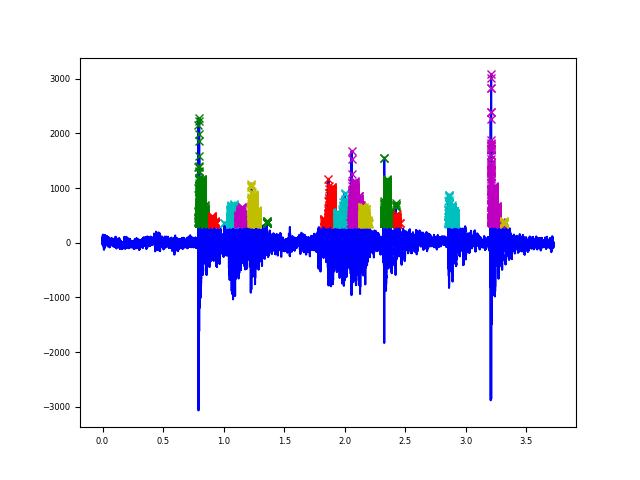
\includegraphics[width=0.8\textwidth]{Images/AcCAPPCHA/hello35_time}
     \caption{\footnotesize{Audio during insertion of password \texttt{hello35} all sub-windows highlighted.}}\label{AcCAPPCHA:hello35_time}
\end{figure}
\subsection{Character correspondence}
When pressed each key of the keyboard produces a variation of the signal, called \textit{press peak}, for a time window of about 8-10 ms\cite{keyboard_acoustic}. This signal trend can also be divided in three consecutive and distinctive areas:
\begin{itemize}
\descItem{touch peak}{peak in a window of 2-3 ms, caused by the finger touching the key}
\item{\textbf{noisy meaningless area}}
\descItem{hit peak}{peak in a window of 2-3 ms, caused by the finger and the key hitting the keyboard supporting plate.}
\end{itemize}
To obtain a prediction of each key pressed by the user, we can extract information from the touch peak, that is the most significant, and the hit peak, that increases the information related to the pression.\\
Following the idea of Asonov and Agrawal, I exploit deep learning to classify each pressed key. In the following sections, there is a detailed explanation of the main phases required and implemented for this classification method:
\begin{itemize}
\item{Data acquisition}
\item{Extraction of features}
\item{Neural network}
\item{Verification}
\end{itemize}

\subsubsection{Data acquisition}
To create a program that record audio while user type something, I created \texttt{DatasetAcquisition.py} source file containing the relative class. After instantiating an object of the class \texttt{AcquireAudio}, it applies \texttt{record} method to this instance.\\
Inside this method, two different program are run in parallel: the first one is a key-logger that is used to classify all the recorded audio files in some directories and the second one that records an audio file during keys typing. The update of private members of the class is guaranteed through the use of the mutual exclusion (mutex) management. The keylogger in the first task requires the access to the operating system signals generated by typing a key on the keyboard. It has the only purpose to continue the acquisition of the audio files even if a special key is pressed (for example F3 button).\\
The choice of running two different tasks in parallel was given by the need of recording audio before the start and after the end of password insertion by the user. Each recorded audio can contain several audio peaks related to multiple insertion of the same key but, during the acquisition of training and test set, I record one audio file for each key pressed.\\
Hence in this particular case, the key-logger waits for the insertion of a single key by the user and then reports it to the thread that performs audio recording. This last task also closes the audio stream and stores the audio signal into a \textit{wav} file named with a progressive number. All the audio files are dynamically organized into a set of subfolders of the output directory, each one with the name of the respective typed key.\\
The recording phase was performed using directly the built-in Realtek microphone and the keyboard of my MSI GL63 8RD laptop. The names of the subfolders/labels, in which each audio file of a pressed key is inserted, are reported in \myref{Appendix}{chapter:KeyMapping}.\\
Looking at Table, we can see that the keylogger changes its behaviour mapping each key to an ASCII string of upper or lower alphabetic characters because otherwise many keys would be mapped into invalid names of folders (for example, the key \textit{'.'} is now mapped into the label \textit{'POINT'}). In the table, there are two columns of labels: the first one related to the label seen by the key-logger, the second one related to the label assigned by me to each key. The reason why these labels differ for some entry are:
\begin{itemize}
\descItem{higher accuracy for spatial distribution of the keys on the keyboard}{for example, \textit{'INSERT'} and \textbf{'0\_INSERT'} (with Num lock on) would be mapped into \textit{'INSERT'} by the key-logger but they are considered different thanks to the final mapping;}
\descItem{improve the classification of keys made by key-logger}{for example, \textit{'ALT'} label is wrongly mapped into \textit{'SHIFT'} by key-logger.}
\descItem{solve the problem of keys mapped only by hardware}{\textit{FN} is the only key with this problem. The key-logger doesn't detect any pressed key, when \textit{FN} is inserted. Hence, I needed to typed it and then another key to be sure that recording for \textit{FN} was performed. Then I made another python script to resize the audio signal and remove the useless second peak.}
\end{itemize}
The last two reasons are very important because they highlight also the power of acoustic side-channel. If an attacker implements an high-level key-logger exploiting also microphone information, the accuracy of its software can increase very much.\\
In fact the hacker could collect a dataset of recordings of pressed keys on the same type of the victim's keyboard and then could train a Neural Network, that will be add in its malicious code. For each key, I record 200 audio signals obtaining a dataset of 20400 audio files. To improve the accuracy of the prediction for the neural network, I performed also Data Augmentation of the audio signals used for the training phase. I tried two approaches: 
\begin{itemize}
\descItem{Time-shift}{from each audio signal I created 4 new audio signals obtained by applying a time-shift respectively of 0.5, 1.0, 1.5 and 2.0 seconds.}
\descItem{Introduction of Gaussian noise}{from each audio signal I added a sequence of random samples from a Gaussian distribution, with standard deviation equal to 150 and mean 0, generating four new audio signals.\\
}
\end{itemize}
Using these approaches I have a training set of 2000 audio signals for key, composed respectively by the following datasets:
\begin{itemize}
\item{200 audio signals manually recorded by me}
\item{800 audio signals obtained by time-shift technique}
\item{800 audio signals from introduction of Gaussian noise}
\end{itemize}
The accuracy of the Neural Network trained on audio signals of both first and second datasets is higher than the one related to the Network trained on first dataset only.  The efficiency of the Neural Network trained on first and third dataset is worst than the one related to the network trained on first dataset only because the third dataset introduces many sequences of FFT coefficients that are very similar even if they are related to different keys. Hence I used only the network trained on the first dataset and both on the first at the second dataset as prediction model. So having 102 keys, I had respectively a dataset of 20400 and 102000 audio files.

\subsubsection{Classification}
I used three different approaches, the first two were taken from the work of Asonov and Agrawal and the last one was based on modern sound classification techniques.\\
Respectively to the method used, the feature for each key was composed by:
\begin{itemize}
\item{FFT coefficients of the touch peak}
\item{FFT coefficients of the hit peak and the touch peak}
\item{Features obtained from the hit peak and the touch peak using a deep learning pre-trained model}
\end{itemize}
In the first two cases, the coefficients are extracted from a window of 3 ms around the peaks and then they are normalized in floating point values in range $[0, 1]$ (see \myref{Figure}{AcCAPPCHA:feature_example}).\\
In the third case, the touch peak and the hit peak samples were concatenated, creating a new signal on which the spectrogram is computed (see \myref{Figure}{AcCAPPCHA:spectrogram}). From the spectrogram, I extract a feature composed by 512 values through the use of VGG16 pre-trained convolutional neural network.\\
In this way, I remove the last fully connected layers, used for classification of other task, and take the intermediate results as feature. The reason of this approach is that a pre-trained network already extracts very well features for classification of a lot of common immages and so it can extract features better than a NN created from scratch.
\begin{figure}[H]
     \centering
     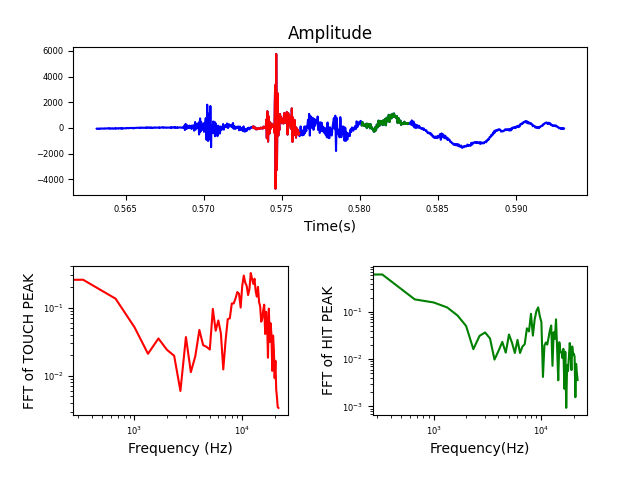
\includegraphics[width=.9\linewidth]{Images/AcCAPPCHA/feature_example}
     \caption{\footnotesize{Example of normalized FFT computation of the touch peak and the hit peak for an audio file of key \textit{'0'}.}}\label{AcCAPPCHA:feature_example}
\end{figure}
\begin{figure}[H]
     \centering
     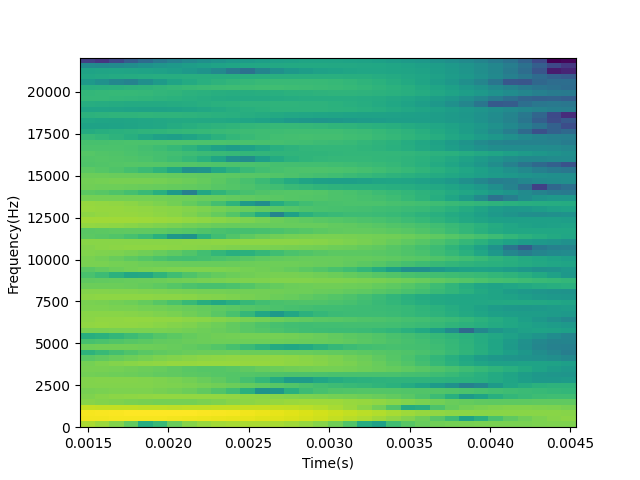
\includegraphics[width=.8\linewidth]{Images/AcCAPPCHA/spectrogram}
     \caption{\footnotesize{Example of spectrogram for an audio file of key \textit{'0'}.}}\label{AcCAPPCHA:spectrogram}
\end{figure}
\clearpage

\subsubsection{Verification}
The audio signal taken, during the insertion of the password, is analysed and then organized in windows as specified in the \myref{Section}{AcCAPPCHA:time_correspondence}, but the verification is based on:
\begin{itemize}
\item{every window previously computed}
\item{the windows that contains the time instants related to the time correspondence}
\end{itemize}
In the first approach the application uses the maximum value of each window as the touch peak and looks for the related hit peak, taking it about 10 ms after the previous peak. After the computation of the features for the two peaks, with one the methods described in the previous section, I perform the prediction using the Neural Network. I collect the most probable predicted keys and I repeat the procedure for every window initially computed on the audio. This method is very weak because after this phase, the algorithm tries to find an ordered sequence of characters, one from each window, that corresponds with the password inserted by the user. If this exists, AcCAPPCHA declares that the user was a human, otherwise a bot. The main problem of this approach is that there is no correspondence in time between a character belonging to the final sequence and the moment in which the same character was inserted physically by the user. In fact there can be false positives caused by the prediction from peak that are not related to the absolute maximum one. In other terms, in the set of the maximuma of all the windows there can be someone that is not related to the touch peak but to a local maximum.\\
The second approach solves the previous problem because the windows, where the maxima are looked for, are obtained by the correspondence time approach. In this case, AcCAPPCHA verification becomes more accurate in theory even if in practice the deep learning technique is not very efficient in prediction for a single key.

\section{Communication between client and server}
The algorithm that perform the evaluation of user activity (see \myref{Section}{AcCAPPCHA:user_activity}) is performed at client side but the value returned by it is evaluated at server-side. The response of the evaluation of user activity concatenated with a nonce and then signed through ECDSA, is sent to the server (see \myref{Section}{inv:communication}). The use of the nonce, unique and random generated sequence, is very important to guarantee that no reply attacks would be performed. In fact the server, after the reception of a message from the client, the server can check if the client has already sent the same nonce before and in this case it declines the message of the client. In this way, any attacker can't reuse a message that previously establishes a client was human. This type of procedure can be also useful to sign HTTP data, for example data sent using POST request (as insertion of password during authentication phase). In the testing phase I performed, I designed and implemented also a simplified version of the communication between the client and the server for an authentication service.\\
The application was tested on local network and the actions performed by involved parties are described in details in the following sections (see Figure ).
\begin{figure}
\centering
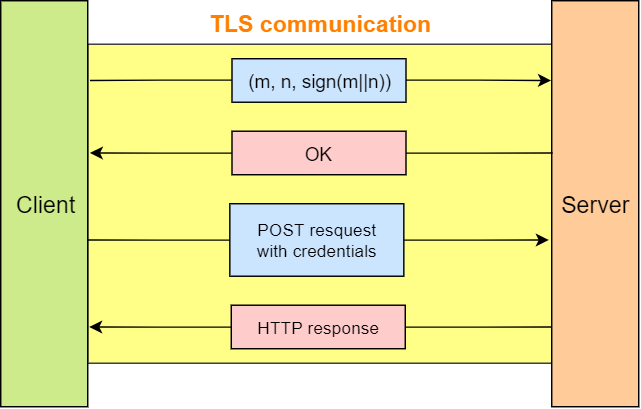
\includegraphics[width=.8\textwidth]{Images/AcCAPPCHA/client-server}
\end{figure}
\subsection{Client}
The client performs the authentication following these steps:
\begin{enumerate}
\item{It establishes a connection with the server over TLS layer to increase the security strength of the communication between the parties;}
\item{It sends the message $(m, n, sign(m||n))$ where:
\begin{itemize}
\item{$m$ is the string with the response of AcCAPPCHA algorithm on client side (\textit{'True'} if Human, \textit{False} if bot)}
\item{$n$ is the the nonce}
\item{$sign(m||n)$ is the ECDSA signature of the concatenation $m||n$ of the response and the nonce. For ECDSA was used SHA256 algorithm.}
\end{itemize}
From a practical point of view, I format the message in the following way:
\begin{table}[H]
\centering\footnotesize
\begin{tabular}{|c|}
\hline
\texttt{m CRLF n sign(m||n)}\\
\hline
\end{tabular}
\end{table}
According to basic rules in grammar of \textbf{HTTP/1.1} (see Section 2.2 of \href{https://tools.ietf.org/html/rfc2616}{RFC 2616}), \textit{CR} is the carriage return ('$\setminus r$') and LF is the line feed ('$\setminus n$'). The spaces in the message aren't considered. In this way, I can separate easily m looking at '$\setminus r\setminus n$'. The nonce has a fixed length of 16 bytes.}
\item{The client waits for response of the server with format:
\begin{table}[H]
\centering\footnotesize
\begin{tabular}{|c|}
\hline
\texttt{response CRLF}\\
\hline
\end{tabular}
\end{table}
If the answer is equal '$OK\setminus r\setminus n$', AcCAPPCHA will go on with the authentication step, otherwise the client-side application performs again the verification, asking again to user to insert the password. The maximum number of trials for a particular user is 3.}
\item{If everything goes well in the previous step, The client sends the credentials (username, password) to the server through a POST request to '/cgi-bin/auth' resource. The name of folder '/cgi-bin' comes from the standard name of the folder with functions and \textit{auth} is the name of the function that server will call. This naming approach was used very much in the past to separate functions code from pure HTML code. The password is not sent directly but it's hashed before using SHA512. The POST request used by the client has the following format:\\
\begin{table}[H]
\hspace{2cm}\centering\footnotesize
\begin{tabular}{|l|}
\hline
\texttt{POST /cgi-bin/auth HTTP/1.1} $\mathtt{\setminus r\setminus n}$\\
\texttt{Host: SP foo.example CRLF}\\
\texttt{Content-Type: SP application/x-www-form-urlencoded CRLF}\\
\texttt{Content-Length: SP SIZE CRLF CRLF}\\
\texttt{user = USERNAME $\mathtt{\&}$ pwd = HASHEDPWD}\\
\hline
\end{tabular}
\end{table}
where everything follows as before the grammar in \href{https://tools.ietf.org/html/rfc2616}{RFC 2616}). In fact also \textbf{SP} represents the space character as in the documentation. \textbf{SIZE}, \textbf{USERNAME} and \textbf{HASHEDPWD} are replaced respectively with the size of the HTTP body, the username of the client and its password hashed with SHA512.
}
\item{The client waits for the HTTP response of the server, containing HTML code as body. Then the client saves the code on the file system and opens the default web browser only to show. The HTML code is intended to show 3 possible scenarios: the user was correctly logged in, the user inserted wrong password, the username wasn't already stored on the server database.}
\end{enumerate}

\subsection{Server}
The client performs the authentication following these steps:
\begin{enumerate}
\item{It establishes a connection with the client, after his request, over TLS layer to increase the security strength of the communication between the parties;}
\item{It receives the message $(m, n, sign(m||n))$ and check the integrity of the message. To do it, the server decrypts the ECDSA signature using the client's ECDSA public key and compares the result with \textit{m||n}.}
\item{If compared messages were the same, the server checks if the nonce was already used by the same client. If so, the server thinks that there was an attacker that is performing a replay attack. If the nonce wasn't already used by the client, it will be stored in a dictionary to monitor clients activity. Each entry of the dictionary is composed by:
\begin{itemize}
\descItem{Key: IP address}{It is the IP address of the client and it is a simplification of the information that identifies a client. For example the client could be associated also to port number used to make the request, the Operating System on which the AcCAPPCHA was running on client-side or other useful parameters.}
\descItem{Value: list of nonces}{Every time a client performs a new verification request on the server, the nonce is added to the list related to its IP address in the dictionary.}
\end{itemize}
}
\item{If the nonce was used for the first time by the client, the server checks the value of the response received by the client. If the response is 'True', the server replies '$OK\setminus r\setminus n$' otherwise '$NO\setminus r\setminus n$'. If some error occurs it sends '$ERROR\setminus r\setminus n$' to the client. In the last two cases, the server terminates.}
\item{If the server doesn't terminate, it waits for the POST request from the client and analyses it to perform authentication service. The server replies to client with several status codes:
\begin{itemize}
\item{\textbf{501 (}Not implemented\textbf{)}\\
If the request is not a POST (e.g. GET)}
\item{\textbf{400 (}Bad Request\textbf{)}\\
If the number of the parameters in the POST body is different from 2 (username and password).}
\item{\textbf{200 (}OK\textbf{)}\\
If the number of the parameters in the POST body is equal to 2, the server will reply with an HTTP response with a body content depending on several cases:
\begin{itemize}
\descItem{User not in the database}{the server sends the following HTML code if the specified username isn't already stored in the database.
\begin{table}[H]
\hspace{2cm}\centering\footnotesize
\begin{tabular}{|p{6cm}|p{0.5cm}c}
\cline{1-1}
\texttt{\key{<!DOCTYPE html>}}&\multirow{7}{*}{
\includegraphics[width=0.5cm]{Images/arrow}}&\multirow{7}{*}{
\includegraphics[scale=0.8]{Images/AcCAPPCHA/no_db_html}}\\
\texttt{\key{<html>}}&&\\
\texttt{\hspace{0.5cm}\key{<body>}}&\\
\texttt{\hspace{1.0cm}\key{<h1>}Failure\key{</h1>}}&&\\
\texttt{\hspace{1.0cm}\key{<p>}First sign up.\key{</p>}}&&\\
\texttt{\hspace{0.5cm}\key{</body>}}&&\\
\texttt{\key{</html>}}&&\\
\cline{1-1}
\end{tabular}
\end{table}
}
\descItem{Wrong password}{the server sends the following HTML code if the hashed password received from the client isn't the same with respect to the one stored in database for the specified username.
\begin{table}[H]
\hspace{2cm}\centering\footnotesize
\begin{tabular}{|p{6cm}|p{0.5cm}c}
\cline{1-1}
\texttt{\key{<!DOCTYPE html>}}&\multirow{7}{*}{
\includegraphics[width=0.5cm]{Images/arrow}}&\multirow{7}{*}{
\includegraphics[scale=0.8]{Images/AcCAPPCHA/failure_html}}\\
\texttt{\key{<html>}}&&\\
\texttt{\hspace{0.5cm}\key{<body>}}&&\\
\texttt{\hspace{1.0cm}\key{<h1>}Failure\key{</h1>}}&&\\
\texttt{\hspace{1.0cm}\key{<p>}Wrong password.\key{</p>}}&&\\
\texttt{\hspace{0.5cm}\key{</body>}}&&\\
\texttt{\key{</html>}}&&\\
\cline{1-1}
\end{tabular}
\end{table}
}
\descItem{User logged in}{the server sends the following HTML code if the specified username exists in the database and  its hashed password stored in the database is the same of the one received through POST request.
\begin{table}[h]
\hspace{2.5cm}\centering\footnotesize
\begin{tabular}{|p{6cm}|p{0.5cm}c}
\cline{1-1}
\texttt{\key{<!DOCTYPE html>}}&\multirow{7}{*}{
\includegraphics[width=0.5cm]{Images/arrow}}&\multirow{7}{*}{
\includegraphics[scale=0.8]{Images/AcCAPPCHA/logged_html}}\\
\texttt{\key{<html>}}&&\\
\texttt{\hspace{0.5cm}\key{<body>}}&&\\
\texttt{\hspace{1.0cm}\key{<h1>}Logged in\key{</h1>}}&&\\
\texttt{\hspace{1.0cm}\key{<p>}Welcome back.\key{</p>}}&&\\
\texttt{\hspace{0.5cm}\key{</body>}}&&\\
\texttt{\key{</html>}}&&\\
\cline{1-1}
\end{tabular}
\end{table}
}
\end{itemize}
}
\end{itemize}
}
\end{enumerate}

\subsection{Database}
The database, created to simulate the search of a username by the server, was made using PostgreSQL. I could store all the information in a simple text file or a csv file but I decide to use this approach to be more flexible to future integration to more complex database.\\
The database is composed by only a table \texttt{CloudUser} to store information about user identity usually stored during the sign up phase. The creation of the database was performed through the following instructions:
\lstset{basicstyle=\footnotesize,breaklines=true}
\lstinputlisting[language=SQL]{../Code/PC/dat/db/db_creation.sql}
I created several domain to manage format of some information of the user. For example the password is a string of 128 characters because each password is hashed using SHA512 and then formatting the result as a string of hexadecimal values.
Then I populated the dataset with some entries, related to fake user, only for testing purpose. An example of inserted users is the following one:
\vspace{0.5cm}
\begin{lstlisting}[language=SQL, showstringspaces=false]
INSERT INTO CloudUser (Name,
                       Surname,
                       Username,
                       Email,
                       Sex,
                       Password)
                       
VALUES ('Raffaele', 
        'Di Nardo Di Maio', 
        'RaffaDNDM', 
        'example1@gmail.com', 
        'Male',
        HASHPASSWORD);
\end{lstlisting}
In practice, \texttt{HASHPASSWORD} is replaced by the string of 128 characters corresponding to the hashed password in hexadecimal format.

\subsection{Encryption Keys}
The creation of the TLS socket for the communication between the client and the server is done by using keys and certificates created thanks to the following bash instructions:
\vspace{0.3cm}
\begin{lstlisting}[language=bash, showstringspaces=false, tabsize=4]
openssl req -new -x509 -days 365 -nodes -out client.pem
		-keyout client.key
\end{lstlisting}
\begin{lstlisting}[language=bash, showstringspaces=false, tabsize=4]
openssl req -new -x509 -days 365 -nodes -out server.pem 
		-keyout server.key
\end{lstlisting}
OpenSSL is a open-source implementation of TLS/SSL protocols and, thanks to the option \texttt{-x509}, you can display certificates and also access to many signing protocols.
In particular, in the previous bash instructions, a X.509 Certificate Signing Request (CSR) is generated and signed for both the parties.\\
Thanks to \texttt{-nodes} the private key is created and not encrypted. The certificates are stored respectively in \textit{server.pem} for the server side and \textit{client.pem} for the client and they are valid for 365 days. The private keys are stored thanks to \texttt{-keyout} option in the \textit{client.pem} and \textit{server.key}.\\\\
The keys, used in ECDSA signing and verification, were created as follow from Python language instead of using a bash tool:
\vspace{0.3cm}
\begin{lstlisting}[language=python, showstringspaces=false, tabsize=4]
from ecdsa import *
from hashlib import sha256

PRIVATE_KEY = SigningKey.generate(curve=SECP256k1,
                                  hashfunc=sha256)

with open('ecdsa.key', 'w') as private_pem:
	private_pem.write(PRIVATE_KEY.to_pem().decode())

PUBLIC_KEY = PRIVATE_KEY.get_verifying_key()

with open('ecdsa.pem', 'w') as public_pem:
	public_pem.write(PUBLIC_KEY.to_pem().decode())
\end{lstlisting}
The \textit{ecdsa} module gives access to the management of operations performed by signing and verification phase. In this case the private key, used to sign a message from the client, was computed on the curve \texttt{SECP256k1} usually used in Bitcoin applications.
\chapter{Experimental results}
All the tests were performed on a MSI GL63 8RD laptop, using Windows 10 Home version 1909 as Operating System.

\section{Human detection}
The application response was tested over all the three possible scenarios (see \myref{Section}{AcCAPPCHA:user_activity}): 
\begin{itemize}
\item{Time correspondence}
\item{Character correspondence}
\item{Both time and character correspondence}
\end{itemize}
The first method is the most efficient and usually at first or second trial already finds a human activity. Sometimes the correspondence isn't found at first trial because of background noise. \\
The last two approaches based on deep learning require the reduction of the number of labels to obtain good results. In this way I limit the possible characters that user could use and the password should be composed of lower case alphabetic characters, accented vowels or numbers (see \myref{Figure}{Results:keyboard}) but considering again the 10 high probable labels predicted for each peak.\\
In any case the last method that uses both the time and the character correspondence speed up the search of the correct peak related to the insertion and reduces the possibility of having a false positive. However there are many false negatives given by the similar sound produces by several keys opposite to D. Asonov, R. Agrawal's conclusions\cite{keyboard_acoustic}.\\
The reasons of their presence could be:
\begin{itemize}
\item{different parts of my keyboard plate produce similar sounds}
\item{the built-in microphone of my laptop is more affected by the noise than an external microphone}
\item{the movements of the user's hands influence the noise during the password insertion}
%WORN OUT = usurato
\item{some keys are more worn out that other}
The worst deep learning method is the one that uses the spectrograms and a pre-trained deep learning model to extract the features of a press peak. In \myref{Table}{}
However during the insertion of the password, the user can obviously type backslash key but then '$\setminus b$' character isn't considered in the final verification.\\

\end{itemize}
\begin{figure}[h]
     \centering
	 \includegraphics[width=0.8\textwidth]{Images/Results/keyboard_less}
     \caption{\footnotesize{Keys to be used in the password (highlighted in green).}}\label{Results:keyboard}
\end{figure}
\begin{table}[h]
\centering
\begin{tabular}{ccc}
\hline
{\textbf{Feature type}}&{\textit{bye5}}&{\textit{hello35}}\\
\hline
\multirow{3}{*}{FFT of touch peak} & {2 (3/4)} & {1}\\
& {2 (3)} & {1}\\
& {1} & {1}\\
\hline
\multirow{3}{*}{FFT of touch and hit peaks} & {2 (3)/4} & {2 (6/7)}\\
& {2 (3/4)} & {1}\\
& {3 (3/4)} & {3 (5.5/7)}\\
\hline
\multirow{3}{*}{Spectrogram of touch and hit peaks} & {NO (3)} & {NO (5.33/7)}\\
& {NO (2.67/4)} & {NO (6/7)}\\
& {NO (2.67/4)} & {NO (4.67/7)}\\
\hline
\end{tabular}
\end{table}

\section{Bot detection}
I've tested both human and bot activities analysing the response generated by AcCAPPCHA. The bot activity was emulated using several approaches and using the username \texttt{'RaffaDNDM'} and its password \textbf{'hello35'}:
\begin{itemize}
\item{\textbf{Python program with} \texttt{popen} \textbf{communication}\\
this approach opens a subprocess and a communication through pipes with stdin and stdout streams (see ). Assuming the hacker obtained the credentials in some way, the bot communicates the username and the password to running AcCAPPCHA with only time correspondence option selected. In practice the strength of AcCAPPCHA against this attack is very high because the insertion of the password is managed through \texttt{getwch()} call in the Windows Operating system. \\
This function belongs to \texttt{msvcrt} module and takes one character at the time. This module guarantees also that the console I/O routines are not compatible with stream I/O or low-level I/O library routines. In the Windows operating systems, the output from these functions is always directed to the console and cannot be redirected through any king of pipes.\\
The program easily accepts the username, because AcCAPPCHA acquires it using standard \texttt{input()} function. Then AcCAPPCHA waits for characters of password, until ENTER key is pressed, but popen doesn't have access to the stream analysed by \texttt{getwch()}. I didn't iterate the insertion of the password for the maximum number of possible trials because even at the first insertion, AcCAPPCHA doesn't see the insertion of the bot.
\begin{lstlisting}[language=python, showstringspaces=false, tabsize=4, basicstyle=\footnotesize, caption={\footnotesize{Bot using popen.}},label={Results:popen_bot}]
from subprocess import Popen
import sys
import msvcrt
from time import sleep

def popen_bot(username, password):
    #Subprocess that redirects pipes
    process = Popen('python3 AcCAPPCHA.py -t -plot',
    				shell=True, 
    				stdin=subprocess.PIPE,
    				stdout=subprocess.PIPE,
    				stderr=subprocess.STDOUT)

    #Wait until username could be inserted
    sleep(4)
    #Write username and password
    credentials = username.encode() + b'\r\n' + \
    			  password.encode() + b'\r\n'
    output = process.communicate(credentials)[0]
    
    print(output.decode())
\end{lstlisting}
}
\item{\textbf{Python program with} \texttt{pynput} \textbf{module}\\
Using this module, I pretended to be a bot and access directly the console, bypassing the stream limits of \textbf{msvcrt} character acquisition. To emulate the user the bot program should start the execution run and immediately after the hacker must open the working terminal with AcCAPPCHA running.\\
This scenario isn't very feasible because requires management of terminal windows but was useful to establish if the insertion of the password by malicious software is correctly classified as a bot activity. Each character of the password is inserted emulating press and release of the corresponding key of the keyboard.
\begin{lstlisting}[language=python, showstringspaces=false, tabsize=4, basicstyle=\footnotesize, caption={\footnotesize{Bot using pynput module.}},label={Results:pynput_bot}]
from pynput.keyboard import Key, Controller
from time import sleep

def input_bot(username, password):
    #Object for control of keyboard events
    keyboard = Controller()

    def press_release(char):
        keyboard.press(char)
        keyboard.release(char)

    #Wait that username could be inserted
    sleep(4)

    #username insertion
    for x in username:
        press_release(x)
    
    press_release(Key.enter)

    #Trials for password insertion
    count = 0
    while(count<3):
        sleep(5)
        
        for x in password:
            press_release(x)

        press_release(Key.enter)
        count += 1
\end{lstlisting}
}
\item{\textbf{Remote control of the PC}\\
the last test was performed by using the program \texttt{Team Viewer} and accessing directly the terminal. For this reason, this type of attack isn't feasible in practice as the previous mentioned attack with Python bot.}
\end{itemize}
In the last two approaches the audio recorded by AcCAPPCHA are very similar and highlights the two most probable situations:
\begin{itemize}
\descItem{The noise during noise evaluation is very high}{If this happens, no audio peaks can be found (see \myref{Figure}{Results:silence_img}).}
\descItem{The noise during noise evaluation is normal or very low}{If this happens, some audio peaks can be found if there is some noise during password insertion. However they don't have time correspondence with time instants stored during the password insertion (see \myref{Figure}{Results:noise_img}). The only case, in which a bot can authenticate it self, is when there is a sequence of audio peaks caused by the noise and the time between them is the same of the stored ones. However this event isn't very probable because it is hard that there would be too high noise only during the insertion of the password and not during the noise evaluation. For example, if the attacker would analyse the background noise finding a sequence of peaks and defining a model for amount of time between each couple of them, he couldn't use information from it. In fact it could insert a character of the password after an amount time previously modelled but in practice, the peaks of background noise would be discarded through noise evaluation.}
\end{itemize}
\begin{figure}[h]
     \centering
	 \begin{subfigure}[b]{0.48\textwidth}
         \centering
         \includegraphics[width=\linewidth]{Images/Results/Bot/silence}
         \caption{\footnotesize{Bot with \texttt{pynput} module.}}
     \end{subfigure}
	 \hfill     
     \begin{subfigure}[b]{0.48\textwidth}
         \centering
         \includegraphics[width=\linewidth]{Images/Results/TeamViewer/silence}
         \caption{\footnotesize{Team Viewer.}}
     \end{subfigure}
     \caption{\footnotesize{Plot of audio during the password insertion with high noise during noise evaluation.}}\label{Results:silence_img}
\end{figure}
\begin{figure}[h]
     \centering
	 \begin{subfigure}[b]{0.48\textwidth}
         \centering
         \includegraphics[width=\linewidth]{Images/Results/Bot/noise}
         \caption{\footnotesize{Bot with \texttt{pynput} module.}}
     \end{subfigure}
	 \hfill     
     \begin{subfigure}[b]{0.48\textwidth}
         \centering
         \includegraphics[width=\linewidth]{Images/Results/TeamViewer/noise}
         \caption{\footnotesize{Team Viewer.}}
     \end{subfigure}
     \caption{\footnotesize{Plot of audio during the password insertion with low noise during noise evaluation.}}\label{Results:noise_img}
\end{figure}

\section{Security analysis}

\chapter{Future work}\label{chapter:Future}
In the future, AcCAPPCHA could be tested on several Operating Systems to make sure that it works correctly on all of them. The application could still be improved by collecting more audio files and increasing the accuracy of the classification approach based on the spectrograms. We can add the management of a blacklist on server side of the AcCAPPCHA to prevent Brute Force attacks and DOS attacks, as explained in \myref{Section}{Results:security}.\\
The most important work that could be added is the implementation of time correspondence approach on smartphones. We can exploit the analysis of audio signals recorded by the microphones of the mobile phones. In fact, many smartphones are now equipped with two microphones and these can be used to increase the accuracy during the research of the audio peaks.\\
Another task that could be added to the mobile version of AcCAPPCHA is the character correspondence. It could exploit the shape of the waves but also the time difference between the two audio peaks, related to the same typed character, and  recorded by the built-in microphones\cite{smartphone_acoustic}. \\
Moreover the voice assistants, like Amazon Echo and Google Home, are becoming increasingly widespread and they are equipped with several microphones. These devices record human activity continuously and only if the user says a specific keyword, they turn on speakers and reply to user. Hence, the audio signals could be exploited to develop new side-channel attacks and analyse input on physical or virtual keyboards\cite{voice_assistant}. Hence the collected information could be exploit to develop also new version of AcCAPPCHA with these devices.\\
VALIDATION SET FOR IMPROVEMENT
\appendix
\chapter{Key Map}\label{appendix:KeyMap}
\begin{figure}[h]
     \centering
     \includegraphics[width=.9\linewidth]{Images/KeyMapping/keyboard}
     \caption{\footnotesize{Layout of the keyboard of my MSI GL63 8RD laptop.}}\label{keymapping:keyboard}
\end{figure}

\renewcommand{\arraystretch}{1.4}
%\setlength{\extrarowheight}{0.05cm}
\footnotesize
\vspace{0.5cm}
\begin{longtable}{|cll|}
\hline
\textbf{Key} & \textbf{Key-logger label} & \textbf{Final label}\\
\hline
\begin{minipage}[c]{.3\textwidth}
\vspace{0.2cm}
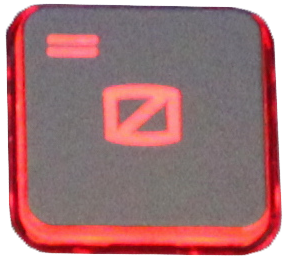
\includegraphics[scale=0.06]{Images/KeyMapping/0}
\vspace{0.2cm}
\end{minipage} & 0 & 0 \\
\hline
\multirow{2}{*}{
\begin{minipage}[c]{.3\textwidth}
\vspace{0.2cm}
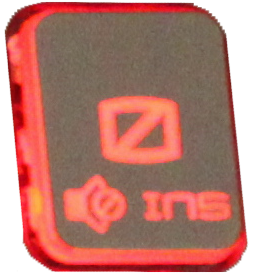
\includegraphics[scale=0.06]{Images/KeyMapping/0_INSERT}
\vspace{0.2cm}
\end{minipage}} & \itemCell{INSERT (Num lock on)} & \multirow{2}{*}{0\_INSERT}\\
& \itemCell{None (Num lock off)} &\\
\hline
\begin{minipage}[c]{.3\textwidth}
\vspace{0.2cm}
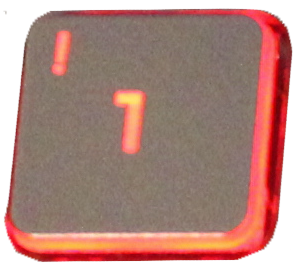
\includegraphics[scale=0.06]{Images/KeyMapping/1}
\vspace{0.2cm}
\end{minipage} & 1 & 1\\
\hline
\multirow{2}{*}{\begin{minipage}[c]{.3\textwidth}
\vspace{0.2cm}
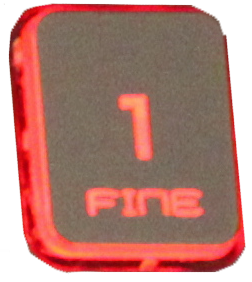
\includegraphics[scale=0.06]{Images/KeyMapping/1_END}
\vspace{0.2cm}
\end{minipage}} & \itemCell{END (Num lock on)} & \multirow{2}{*}{1\_END}\\
& \itemCell{None (Num lock off)} &\\
\hline
\begin{minipage}[c]{.3\textwidth}
\vspace{0.2cm}
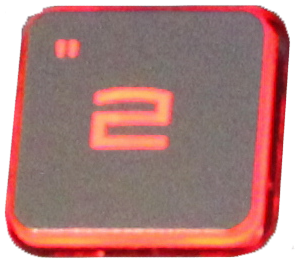
\includegraphics[scale=0.06]{Images/KeyMapping/2}
\vspace{0.2cm}
\end{minipage} & 2 & 2\\
\hline
\multirow{2}{*}{\begin{minipage}[c]{.3\textwidth}
\vspace{0.2cm}
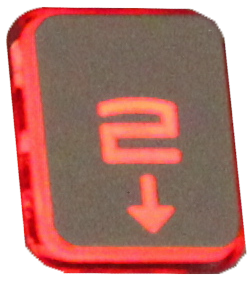
\includegraphics[scale=0.06]{Images/KeyMapping/2_DOWN}
\vspace{0.2cm}
\end{minipage}} & \itemCell{DOWN (Num lock on)} & \multirow{2}{*}{2\_DOWN}\\
& \itemCell{None (Num lock off)} &\\
\hline
\begin{minipage}[c]{.3\textwidth}
\vspace{0.2cm}
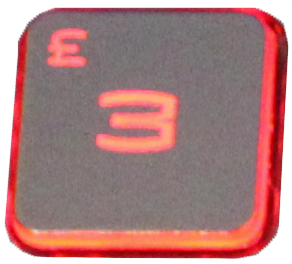
\includegraphics[scale=0.06]{Images/KeyMapping/3}
\vspace{0.2cm}
\end{minipage} & 3 & 3\\
\hline
\multirow{2}{*}{\begin{minipage}[c]{.3\textwidth}
\vspace{0.2cm}
\includegraphics[scale=0.06]{Images/KeyMapping/3_PAGE_DOWN}
\vspace{0.2cm}
\end{minipage}} & \itemCell{PAGE\_DOWN (Num lock on)} & \multirow{2}{*}{3\_PAGE\_DOWN}\\
& \itemCell{None (Num lock off)} &\\
\hline
\begin{minipage}[c]{.3\textwidth}
\vspace{0.2cm}
\includegraphics[scale=0.06]{Images/KeyMapping/4}
\vspace{0.2cm}
\end{minipage} & 4 & 4\\
\hline
\multirow{2}{*}{\begin{minipage}[c]{.3\textwidth}
\vspace{0.2cm}
\includegraphics[scale=0.06]{Images/KeyMapping/4_LEFT}
\vspace{0.2cm}
\end{minipage}} & \itemCell{LEFT (Num lock on)} & \multirow{2}{*}{4\_LEFT}\\
& \itemCell{None (Num lock off)} &\\
\hline
\begin{minipage}[c]{.3\textwidth}
\vspace{0.2cm}
\includegraphics[scale=0.06]{Images/KeyMapping/5}
\vspace{0.2cm}
\end{minipage} & 5 & 5\\
\hline
\multirow{2}{*}{\begin{minipage}[c]{.3\textwidth}
\vspace{0.2cm}
\includegraphics[scale=0.06]{Images/KeyMapping/5_NUM}
\vspace{0.2cm}
\end{minipage}} & \itemCell{None (Num lock on)} & \multirow{2}{*}{5\_NUM}\\
& \itemCell{None (Num lock off)} &\\
\hline
\begin{minipage}[c]{.3\textwidth}
\vspace{0.2cm}
\includegraphics[scale=0.06]{Images/KeyMapping/6}
\vspace{0.2cm}
\end{minipage} & 6 & 6\\
\hline
\multirow{2}{*}{\begin{minipage}[c]{.3\textwidth}
\vspace{0.2cm}
\includegraphics[scale=0.06]{Images/KeyMapping/6_RIGHT}
\vspace{0.2cm}
\end{minipage}} & \itemCell{RIGHT (Num lock on)} & \multirow{2}{*}{6\_RIGHT}\\
& \itemCell{None (Num lock off)} &\\
\hline
\begin{minipage}[c]{.3\textwidth}
\vspace{0.2cm}
\includegraphics[scale=0.06]{Images/KeyMapping/7}
\vspace{0.2cm}
\end{minipage} & 7 & 7\\
\hline
\multirow{2}{*}{\begin{minipage}[c]{.3\textwidth}
\vspace{0.2cm}
\includegraphics[scale=0.06]{Images/KeyMapping/7_HOME}
\vspace{0.2cm}
\end{minipage}} & \itemCell{HOME (Num lock on)} & \multirow{2}{*}{7\_HOME}\\
& \itemCell{None (Num lock off)} &\\
\hline
\begin{minipage}[c]{.3\textwidth}
\vspace{0.2cm}
\includegraphics[scale=0.06]{Images/KeyMapping/8}
\vspace{0.2cm}
\end{minipage} & 8 & 8\\
\hline
\multirow{2}{*}{\begin{minipage}[c]{.3\textwidth}
\vspace{0.2cm}
\includegraphics[scale=0.06]{Images/KeyMapping/8_UP}
\vspace{0.2cm}
\end{minipage}} & \itemCell{UP (Num lock on)} & \multirow{2}{*}{8\_UP}\\
& \itemCell{None (Num lock off)} &\\
\hline
\begin{minipage}[c]{.3\textwidth}
\vspace{0.2cm}
\includegraphics[scale=0.06]{Images/KeyMapping/9}
\vspace{0.2cm}
\end{minipage} & 9 & 9\\
\hline
\multirow{2}{*}{\begin{minipage}[c]{.3\textwidth}
\vspace{0.2cm}
\includegraphics[scale=0.06]{Images/KeyMapping/9_PAGE_UP}
\vspace{0.2cm}
\end{minipage}} & \itemCell{PAGE\_UP (Num lock on)} & \multirow{2}{*}{9\_PAGE\_UP}\\
& \itemCell{None (Num lock off)} &\\
\hline
\begin{minipage}[c]{.3\textwidth}
\vspace{0.2cm}
\includegraphics[scale=0.06]{Images/KeyMapping/a}
\vspace{0.2cm}
\end{minipage} & a & a\\
\hline
\begin{minipage}[c]{.3\textwidth}
\vspace{0.2cm}
\includegraphics[scale=0.06]{Images/KeyMapping/ALT}
\vspace{0.2cm}
\end{minipage} & SHIFT & ALT\\
\hline
\begin{minipage}[c]{.3\textwidth}
\vspace{0.2cm}
\includegraphics[scale=0.06]{Images/KeyMapping/ALT_GR}
\vspace{0.2cm}
\end{minipage} & CTRL & ALT\_GR\\
\hline
\begin{minipage}[c]{.3\textwidth}
\vspace{0.2cm}
\includegraphics[scale=0.06]{Images/KeyMapping/APOSTROPHE}
\vspace{0.2cm}
\end{minipage} & APOSTROPHE & APOSTROPHE\\
\hline
\begin{minipage}[c]{.3\textwidth}
\vspace{0.2cm}
\includegraphics[scale=0.06]{Images/KeyMapping/b}
\vspace{0.2cm}
\end{minipage} & b & b\\
\hline
\begin{minipage}[c]{.3\textwidth}
\vspace{0.2cm}
\includegraphics[scale=0.06]{Images/KeyMapping/BACKSLASH}
\vspace{0.2cm}
\end{minipage} & BACKSLASH & BACKSLASH\\
\hline
\begin{minipage}[c]{.3\textwidth}
\vspace{0.2cm}
\includegraphics[scale=0.06]{Images/KeyMapping/BACKSPACE}
\vspace{0.2cm}
\end{minipage} & BACKSPACE & BACKSPACE\\
\hline
\begin{minipage}[c]{.3\textwidth}
\vspace{0.2cm}
\includegraphics[scale=0.06]{Images/KeyMapping/c}
\vspace{0.2cm}
\end{minipage} & c & c\\
\hline
\begin{minipage}[c]{.3\textwidth}
\vspace{0.2cm}
\includegraphics[scale=0.06]{Images/KeyMapping/CAPS_LOCK}
\vspace{0.2cm}
\end{minipage} & CAPS\_LOCK & CAPS\_LOCK\\
\hline
\begin{minipage}[c]{.3\textwidth}
\vspace{0.2cm}
\includegraphics[scale=0.06]{Images/KeyMapping/COMMA}
\vspace{0.2cm}
\end{minipage} & COMMA & COMMA\\
\hline
\begin{minipage}[c]{.3\textwidth}
\vspace{0.2cm}
\includegraphics[scale=0.06]{Images/KeyMapping/CTRL}
\vspace{0.2cm}
\end{minipage} & CTRL & CTRL\\
\hline
\begin{minipage}[c]{.3\textwidth}
\vspace{0.2cm}
\includegraphics[scale=0.06]{Images/KeyMapping/CTRL_R}
\vspace{0.2cm}
\end{minipage} & CTRL\_R & CTRL\_R\\
\hline
\begin{minipage}[c]{.3\textwidth}
\vspace{0.2cm}
\includegraphics[scale=0.06]{Images/KeyMapping/d}
\vspace{0.2cm}
\end{minipage} & d & d\\
\hline
\begin{minipage}[c]{.3\textwidth}
\vspace{0.2cm}
\includegraphics[scale=0.06]{Images/KeyMapping/DELETE}
\vspace{0.2cm}
\end{minipage} & DELETE & DELETE\\
\hline
\begin{minipage}[c]{.3\textwidth}
\vspace{0.2cm}
\includegraphics[scale=0.06]{Images/KeyMapping/DOWN}
\vspace{0.2cm}
\end{minipage} & DOWN & DOWN\\
\hline
\begin{minipage}[c]{.3\textwidth}
\vspace{0.2cm}
\includegraphics[scale=0.06]{Images/KeyMapping/e}
\vspace{0.2cm}
\end{minipage} & e & e\\
\hline
\begin{minipage}[c]{.3\textwidth}
\vspace{0.2cm}
\includegraphics[scale=0.06]{Images/KeyMapping/ENTER}
\vspace{0.2cm}
\end{minipage} & ENTER & ENTER\\
\hline
\begin{minipage}[c]{.3\textwidth}
\vspace{0.2cm}
\includegraphics[scale=0.06]{Images/KeyMapping/ENTER_R}
\vspace{0.2cm}
\end{minipage} & ENTER & ENTER\_R\\
\hline
\begin{minipage}[c]{.3\textwidth}
\vspace{0.2cm}
\includegraphics[scale=0.06]{Images/KeyMapping/ESC}
\vspace{0.2cm}
\end{minipage} & ESC & ESC\\
\hline
\begin{minipage}[c]{.3\textwidth}
\vspace{0.2cm}
\includegraphics[scale=0.06]{Images/KeyMapping/f}
\vspace{0.2cm}
\end{minipage} & f & f\\
\hline
\begin{minipage}[c]{.3\textwidth}
\vspace{0.2cm}
\includegraphics[scale=0.06]{Images/KeyMapping/F1}
\vspace{0.2cm}
\end{minipage} & F1 & F1\\
\hline
\begin{minipage}[c]{.3\textwidth}
\vspace{0.2cm}
\includegraphics[scale=0.06]{Images/KeyMapping/F2}
\vspace{0.2cm}
\end{minipage} & F2 & F2\\
\hline
\begin{minipage}[c]{.3\textwidth}
\vspace{0.2cm}
\includegraphics[scale=0.06]{Images/KeyMapping/F3}
\vspace{0.2cm}
\end{minipage} & F3 & F3\\
\hline
\begin{minipage}[c]{.3\textwidth}
\vspace{0.2cm}
\includegraphics[scale=0.06]{Images/KeyMapping/F4}
\vspace{0.2cm}
\end{minipage} & F4 & F4\\
\hline
\begin{minipage}[c]{.3\textwidth}
\vspace{0.2cm}
\includegraphics[scale=0.06]{Images/KeyMapping/F5}
\vspace{0.2cm}
\end{minipage} & F5 & F5\\
\hline
\begin{minipage}[c]{.3\textwidth}
\vspace{0.2cm}
\includegraphics[scale=0.06]{Images/KeyMapping/F6}
\vspace{0.2cm}
\end{minipage} & F6 & F6\\
\hline
\begin{minipage}[c]{.3\textwidth}
\vspace{0.2cm}
\includegraphics[scale=0.06]{Images/KeyMapping/F7}
\vspace{0.2cm}
\end{minipage} & F7 & F7\\
\hline
\begin{minipage}[c]{.3\textwidth}
\vspace{0.2cm}
\includegraphics[scale=0.06]{Images/KeyMapping/F8}
\vspace{0.2cm}
\end{minipage} & F8 & F8\\
\hline
\begin{minipage}[c]{.3\textwidth}
\vspace{0.2cm}
\includegraphics[scale=0.06]{Images/KeyMapping/F9}
\vspace{0.2cm}
\end{minipage} & F9 & F9\\
\hline
\begin{minipage}[c]{.3\textwidth}
\vspace{0.2cm}
\includegraphics[scale=0.06]{Images/KeyMapping/F10}
\vspace{0.2cm}
\end{minipage} & F10 & F10\\
\hline
\begin{minipage}[c]{.3\textwidth}
\vspace{0.2cm}
\includegraphics[scale=0.06]{Images/KeyMapping/F11}
\vspace{0.2cm}
\end{minipage} & F11 & F11\\
\hline
\begin{minipage}[c]{.3\textwidth}
\vspace{0.2cm}
\includegraphics[scale=0.06]{Images/KeyMapping/F12}
\vspace{0.2cm}
\end{minipage} & F12 & F12\\
\hline
\begin{minipage}[c]{.3\textwidth}
\vspace{0.2cm}
\includegraphics[scale=0.06]{Images/KeyMapping/FN}
\vspace{0.2cm}
\end{minipage} &  & FN\\
\hline
\begin{minipage}[c]{.3\textwidth}
\vspace{0.2cm}
\includegraphics[scale=0.06]{Images/KeyMapping/g}
\vspace{0.2cm}
\end{minipage} & g & g\\
\hline
\begin{minipage}[c]{.3\textwidth}
\vspace{0.2cm}
\includegraphics[scale=0.06]{Images/KeyMapping/h}
\vspace{0.2cm}
\end{minipage} & h & h\\
\hline
\begin{minipage}[c]{.3\textwidth}
\vspace{0.2cm}
\includegraphics[scale=0.06]{Images/KeyMapping/i}
\vspace{0.2cm}
\end{minipage} & i & i\\
\hline
\begin{minipage}[c]{.3\textwidth}
\vspace{0.2cm}
\includegraphics[scale=0.06]{Images/KeyMapping/INSERT}
\vspace{0.2cm}
\end{minipage} & INSERT & INSERT\\
\hline
\begin{minipage}[c]{.3\textwidth}
\vspace{0.2cm}
\includegraphics[scale=0.06]{Images/KeyMapping/j}
\vspace{0.2cm}
\end{minipage} & j & j\\
\hline
\begin{minipage}[c]{.3\textwidth}
\vspace{0.2cm}
\includegraphics[scale=0.06]{Images/KeyMapping/k}
\vspace{0.2cm}
\end{minipage} & k & k\\
\hline
\begin{minipage}[c]{.3\textwidth}
\vspace{0.2cm}
\includegraphics[scale=0.06]{Images/KeyMapping/l}
\vspace{0.2cm}
\end{minipage} & l & l\\
\hline
\begin{minipage}[c]{.3\textwidth}
\vspace{0.2cm}
\includegraphics[scale=0.06]{Images/KeyMapping/LEFT}
\vspace{0.2cm}
\end{minipage} & LEFT & LEFT\\
\hline
\begin{minipage}[c]{.3\textwidth}
\vspace{0.2cm}
\includegraphics[scale=0.06]{Images/KeyMapping/LOWER}
\vspace{0.2cm}
\end{minipage} & LOWER & LOWER\\
\hline
\begin{minipage}[c]{.3\textwidth}
\vspace{0.2cm}
\includegraphics[scale=0.06]{Images/KeyMapping/m}
\vspace{0.2cm}
\end{minipage} & m & m\\
\hline
\begin{minipage}[c]{.3\textwidth}
\vspace{0.2cm}
\includegraphics[scale=0.06]{Images/KeyMapping/MINUS}
\vspace{0.2cm}
\end{minipage} & MINUS & MINUS\\
\hline
\begin{minipage}[c]{.3\textwidth}
\vspace{0.2cm}
\includegraphics[scale=0.06]{Images/KeyMapping/MINUS_R}
\vspace{0.2cm}
\end{minipage} & MINUS & MINUS\_R\\
\hline
\begin{minipage}[c]{.3\textwidth}
\vspace{0.2cm}
\includegraphics[scale=0.06]{Images/KeyMapping/n}
\vspace{0.2cm}
\end{minipage} & n & n\\
\hline
\begin{minipage}[c]{.3\textwidth}
\vspace{0.2cm}
\includegraphics[scale=0.06]{Images/KeyMapping/NUM_LOCK}
\vspace{0.2cm}
\end{minipage} & NUM\_LOCK & NUM\_LOCK\\
\hline
\begin{minipage}[c]{.3\textwidth}
\vspace{0.2cm}
\includegraphics[scale=0.06]{Images/KeyMapping/o}
\vspace{0.2cm}
\end{minipage} & o & o\\
\hline
\begin{minipage}[c]{.3\textwidth}
\vspace{0.2cm}
\includegraphics[scale=0.06]{Images/KeyMapping/p}
\vspace{0.2cm}
\end{minipage} & p & p\\
\hline
\begin{minipage}[c]{.3\textwidth}
\vspace{0.2cm}
\includegraphics[scale=0.06]{Images/KeyMapping/PAGE_DOWN}
\vspace{0.2cm}
\end{minipage} & PAGE\_DOWN & PAGE\_DOWN\\
\hline
\begin{minipage}[c]{.3\textwidth}
\vspace{0.2cm}
\includegraphics[scale=0.06]{Images/KeyMapping/PAGE_UP}
\vspace{0.2cm}
\end{minipage} & PAGE\_UP & PAGE\_UP\\
\hline
\begin{minipage}[c]{.3\textwidth}
\vspace{0.2cm}
\includegraphics[scale=0.06]{Images/KeyMapping/PAUSE}
\vspace{0.2cm}
\end{minipage} & PAUSE & PAUSE\\
\hline
\begin{minipage}[c]{.3\textwidth}
\vspace{0.2cm}
\includegraphics[scale=0.06]{Images/KeyMapping/PLUS}
\vspace{0.2cm}
\end{minipage} & PLUS & PLUS\\
\hline
\begin{minipage}[c]{.3\textwidth}
\vspace{0.2cm}
\includegraphics[scale=0.06]{Images/KeyMapping/PLUS_R}
\vspace{0.2cm}
\end{minipage} & PLUS & PLUS\_R\\
\hline
\begin{minipage}[c]{.3\textwidth}
\vspace{0.2cm}
\includegraphics[scale=0.06]{Images/KeyMapping/POINT}
\vspace{0.2cm}
\end{minipage} & POINT & POINT\\
\hline
\multirow{2}{*}{\begin{minipage}[c]{.3\textwidth}
\vspace{0.2cm}
\includegraphics[scale=0.06]{Images/KeyMapping/9_PAGE_UP}
\vspace{0.2cm}
\end{minipage}} & \itemCell{DELETE (Num lock on)} & \multirow{2}{*}{POINT\_DELETE}\\
& \itemCell{None (Num lock off)} &\\
\hline
\begin{minipage}[c]{.3\textwidth}
\vspace{0.2cm}
\includegraphics[scale=0.06]{Images/KeyMapping/PRINT_SCREEN}
\vspace{0.2cm}
\end{minipage} & PRINT\_SCREEN & PRINT\_SCREEN\\
\hline
\begin{minipage}[c]{.3\textwidth}
\vspace{0.2cm}
\includegraphics[scale=0.06]{Images/KeyMapping/q}
\vspace{0.2cm}
\end{minipage} & q & q\\
\hline
\begin{minipage}[c]{.3\textwidth}
\vspace{0.2cm}
\includegraphics[scale=0.06]{Images/KeyMapping/r}
\vspace{0.2cm}
\end{minipage} & r & r\\
\hline
\begin{minipage}[c]{.3\textwidth}
\vspace{0.2cm}
\includegraphics[scale=0.06]{Images/KeyMapping/RIGHT}
\vspace{0.2cm}
\end{minipage} & RIGHT & RIGHT\\
\hline
\begin{minipage}[c]{.3\textwidth}
\vspace{0.2cm}
\includegraphics[scale=0.06]{Images/KeyMapping/s}
\vspace{0.2cm}
\end{minipage} & s & s\\
\hline
\begin{minipage}[c]{.3\textwidth}
\vspace{0.2cm}
\includegraphics[scale=0.06]{Images/KeyMapping/SCROLL_LOCK}
\vspace{0.2cm}
\end{minipage} & SCROLL\_LOCK & SCROLL\_LOCK\\
\hline
\begin{minipage}[c]{.3\textwidth}
\vspace{0.2cm}
\includegraphics[scale=0.06]{Images/KeyMapping/SHIFT}
\vspace{0.2cm}
\end{minipage} & SHIFT & SHIFT\\
\hline
\begin{minipage}[c]{.3\textwidth}
\vspace{0.2cm}
\includegraphics[scale=0.06]{Images/KeyMapping/SHIFT_R}
\vspace{0.2cm}
\end{minipage} & SHIFT & SHIFT\_R\\
\hline
\begin{minipage}[c]{.3\textwidth}
\vspace{0.2cm}
\includegraphics[scale=0.06]{Images/KeyMapping/SLASH}
\vspace{0.2cm}
\end{minipage} & MINUS & SLASH\\
\hline
\begin{minipage}[c]{.3\textwidth}
\vspace{0.2cm}
\includegraphics[scale=0.06]{Images/KeyMapping/SPACE}
\vspace{0.2cm}
\end{minipage} & SPACE & SPACE\\
\hline
\begin{minipage}[c]{.3\textwidth}
\vspace{0.2cm}
\includegraphics[scale=0.06]{Images/KeyMapping/STAR}
\vspace{0.2cm}
\end{minipage} & STAR & STAR\\
\hline
\begin{minipage}[c]{.3\textwidth}
\vspace{0.2cm}
\includegraphics[scale=0.06]{Images/KeyMapping/t}
\vspace{0.2cm}
\end{minipage} & t & t\\
\hline
\begin{minipage}[c]{.3\textwidth}
\vspace{0.2cm}
\includegraphics[scale=0.06]{Images/KeyMapping/TAB}
\vspace{0.2cm}
\end{minipage} & TAB & TAB\\
\hline
\begin{minipage}[c]{.3\textwidth}
\vspace{0.2cm}
\includegraphics[scale=0.06]{Images/KeyMapping/u}
\vspace{0.2cm}
\end{minipage} & u & u\\
\hline
\begin{minipage}[c]{.3\textwidth}
\vspace{0.2cm}
\includegraphics[scale=0.06]{Images/KeyMapping/UP}
\vspace{0.2cm}
\end{minipage} & UP & UP\\
\hline
\begin{minipage}[c]{.3\textwidth}
\vspace{0.2cm}
\includegraphics[scale=0.06]{Images/KeyMapping/v}
\vspace{0.2cm}
\end{minipage} & v & v\\
\hline
\begin{minipage}[c]{.3\textwidth}
\vspace{0.2cm}
\includegraphics[scale=0.06]{Images/KeyMapping/w}
\vspace{0.2cm}
\end{minipage} & w & w\\
\hline
\begin{minipage}[c]{.3\textwidth}
\vspace{0.2cm}
\includegraphics[scale=0.06]{Images/KeyMapping/WINDOWS}
\vspace{0.2cm}
\end{minipage} & SHIFT & WINDOWS\\
\hline
\begin{minipage}[c]{.3\textwidth}
\vspace{0.2cm}
\includegraphics[scale=0.06]{Images/KeyMapping/x}
\vspace{0.2cm}
\end{minipage} & x & x\\
\hline
\begin{minipage}[c]{.3\textwidth}
\vspace{0.2cm}
\includegraphics[scale=0.06]{Images/KeyMapping/y}
\vspace{0.2cm}
\end{minipage} & y & y\\
\hline
\begin{minipage}[c]{.3\textwidth}
\vspace{0.2cm}
\includegraphics[scale=0.06]{Images/KeyMapping/z}
\vspace{0.2cm}
\end{minipage} & z & z\\
\hline
\begin{minipage}[c]{.3\textwidth}
\vspace{0.2cm}
\includegraphics[scale=0.06]{Images/KeyMapping/à}
\vspace{0.2cm}
\end{minipage} & à & à\\
\hline
\begin{minipage}[c]{.3\textwidth}
\vspace{0.2cm}
\includegraphics[scale=0.06]{Images/KeyMapping/è}
\vspace{0.2cm}
\end{minipage} & è & è\\
\hline
\begin{minipage}[c]{.3\textwidth}
\vspace{0.2cm}
\includegraphics[scale=0.06]{Images/KeyMapping/ì}
\vspace{0.2cm}
\end{minipage} & ì & ì\\
\hline
\begin{minipage}[c]{.3\textwidth}
\vspace{0.2cm}
\includegraphics[scale=0.06]{Images/KeyMapping/ò}
\vspace{0.2cm}
\end{minipage} & ò & ò\\
\hline
\begin{minipage}[c]{.3\textwidth}
\vspace{0.2cm}
\includegraphics[scale=0.06]{Images/KeyMapping/ù}
\vspace{0.2cm}
\end{minipage} & ù & ù\\
\hline
\caption{Map of pressed key performed by key-logger and then manually modified in final label.}
\end{longtable}
\normalsize

\chapter{Program}\label{appendix:Program}
In the following sections, I describe the command line parameters of the main programs, developed to perform AcCAPPCHA verification. As explained in the previous chapters, all the code was developed using the \texttt{Python} programming language.

\section{DatasetAcquisition.py}
\texttt{DatasetAcquisition.py} does several actions: the recording of the audio during the insertion of a key, the plotting of the graphics of the audio files, the extraction of the features from the audio peak in each audio files. The audio recording terminates after a number of key presses. The label related to first key press defines the name of the subfolder of the output path where the wav file will be stored. By default the program waits only for sequences of 1 key and then stores it.

{\footnotesize
\begin{longtable}{rl}
\hline
\textbf{Parameter} & \textbf{Description}\\
\hline
\texttt{-plot} & If specified, the program plots data already acquired instead of\\
\texttt{-p} & new acquired audio files\\
&\\
\texttt{-record} & If specified, the program records audio while the keylogger is going on\\
\texttt{-r} &\\
&\\
\texttt{-extract} & If specified, the program extracts features from audio already recorded\\
\texttt{-e} &\\
&\\
&\\
\texttt{-zoom} & If specified, the program plots the audio peaks of the input files in\\
\texttt{-z} & graphic images, showing only the signal in the neighbourhood of the peak.\\
&\\
\texttt{-file} \textit{path} & It specifies the \textit{path} of the file that you want to plot\\
\texttt{-f} \textit{path} & or from which you want to extract features\\
&\\
\texttt{-dir} \textit{path} & It specifies, it is the \textit{path} the folder where:\\
\texttt{-d} \textit{path} & \itemCellTab{\textbf{-r option}}\\
& \hspace{0.8cm}there will be stored audio files acquired from the work\\
& \hspace{0.8cm}of both the recorder and the keylogger\\
&\itemCellTab{\textbf{-p option and -e option}}\\
& \hspace{0.8cm}there are already recored audio files on which the\\
& \hspace{0.8cm}extraction and the plotting will be applied\\
&\\
\texttt{-out} \textit{path} & It specifies the \textit{path} of the output folder\\
\texttt{-o} \textit{path} & in which the graphics will be stored as \textit{path}\\
& images (if \texttt{-p/-plot} selected)\\
\hline
\end{longtable}}

\section{AcCAPPCHA.py}
\texttt{AcCAPPCHA.py} runs at the client side and it performs the verification of the user identity, using either time or character correspondence. Then it sends the results to the server and communicates with it during the authentication phase.

{\footnotesize
\begin{longtable}{rl}
\hline
\textbf{Parameter} & \textbf{Description}\\
\hline
\texttt{-dir} \textit{path} & It specifies the \textit{path} of the folder with the\\
\texttt{-d} \textit{path} & 3 subfolders: 'touch/', 'touch\_hit/' and 'spectrum/'.\\
& Each of them contains a folder called 'model/' that contains the information\\
& of the pre-trained network that classifies the keys of the keyboard.\\
& It's mandatory if -deep/-dl option is specified.\\
&\\
\texttt{-time} & If specified, AcCAPPCHA performs the time correspondence.\\
\texttt{-t} & \\
&\\
&\\
\texttt{-deep} & If specified, AcCAPPCHA performs the character correspondence.\\
\texttt{-dl} & \\
&\\
\texttt{-plot} & If specified, AcCAPPCHA plots the graphics of the peaks in the\\
\texttt{-p} & audio signal recorded during the password insertion.\\
&\\
\texttt{-debug} & If specified, AcCAPPCHA shows debug information about the\\
\texttt{-dbg} & verification phases\\
\hline
\end{longtable}}

\section{Authentication.py}
\texttt{Authentication.py} runs forever at the server side. It performs the verification of the message received by the client and it accesses the database during the authentication phase.
\begin{table}[h]
\centering\footnotesize
\begin{tabular}{rl}
\hline
\textbf{Parameter} & \textbf{Description}\\
\hline
\texttt{-debug} & If specified, the program shows debug information about the remote client\\
\texttt{-dbg} &\\
\hline
\end{tabular}
\end{table}
\begin{thebibliography}{9}
\bibitem{DECAPTCHA} E. Bursztein, M. Martin, and J. Mitchell, "Text-based CAPTCHA strengths and weaknesses" in \emph{Proc. 18th ACM Conf. Comput. Commun. Secur. (CCS), 2011, pp. 125–138.}

\bibitem{Improved_AUDIO} Jennifer Tam, Jiri Simsa, David Huggins-Daines, Luis von Ahn, and Manuel Blum, "Improving Audio CAPTCHAs" in \emph{Symposium On Usable Privacy and Security (SOUPS), 2008.}

\bibitem{TEXT_AUDIO} Sarika Choudhary, Ritika Saroha, Yatan Dahiya, and Sachin Choudhary, "Understanding CAPTCHA: Text and Audio Based Captcha with its Applications" in \emph{International Journal of Advanced Research in Computer Science and Software Engineering vol. 3 (6), pp. 106-115, June-2013.}

\end{thebibliography}
\chapter*{Acknowledgements}
Professor Migliardi\\\\
I would like to express my very great appreciation to Dr Guerar\\\\
I would like to express my gratitude to University of Padova for the study path I performed. The uncertainty about the future and the idea of being far from needed cyber security skills have become a stimulus to improve myself. I learn a lot and I got hooked on the programming, starting from zero level of it, thanks to the professors' professionalism and knowledge. During the last five years, I've changed and now I spend programming all my free time. Thanks to University because professors follow my thirst of knowledge and I grew up, living alone and really becoming an adult.\\\\
Thanks to staff,\\\\
Thanks to other company,\\\\
I would like to express my gratitude to my family that taught me to never give up. In particular thank to my sister that, with her great experience in University course, has been a reference for my study attitude and perseverance.\\\\
Thanks to my grandmother Concetta that, with her smiles, has left to me happiness during my darker and difficult periods.\\\\
Thanks to my grandmother Maria that, was always worried for my health issues and tries always to give me up using her food. \\\\
Thanks to Cristina,\\\\
Thanks to Francesca, because even if we had many commitments we have always found 5 minutes to stay together and to support the other one in his/her choices.\\\\
Thanks to Davide,\\\\
Thanks to Giuseppe, Aurora, Alessia and Sara,\\\\
Thanks to Elia,\\\\
Thanks to Lorenzo,\\\\

\end{document}